\documentclass[conference, letterpaper]{IEEEtran}

\ifCLASSINFOpdf
   \usepackage[pdftex]{graphicx}
\else
\fi

\usepackage[cmex10]{amsmath}
\usepackage{amssymb}
\usepackage{color}
\usepackage{fancyhdr}
\usepackage[caption=false, font=footnotesize]{subfig}
\usepackage{booktabs}
\usepackage{array}
\usepackage{tabularx}
\usepackage{multirow}
\newcolumntype{C}{>{\centering\arraybackslash}X}
\usepackage{url}
\usepackage{orcidlink}
\usepackage{threeparttable}
\usepackage{dblfloatfix}

% Relax float placement so wide (double-column) tables can sit near their text
\setcounter{topnumber}{3}
\setcounter{dbltopnumber}{3}
\renewcommand{\topfraction}{0.95}
\renewcommand{\dbltopfraction}{0.95}
\renewcommand{\textfraction}{0.05}
\renewcommand{\floatpagefraction}{0.85}
\renewcommand{\dblfloatpagefraction}{0.85}

\hyphenation{tu-ber-cu-lo-sis ra-di-o-graph}

% absorb minor bibliography overflow (long titles/URLs) without ragged spacing warnings
\setlength{\emergencystretch}{3em}

\renewcommand{\thispagestyle}[1]{}

\fancypagestyle{plain}{
        \fancyhead{}
        \fancyhead[C]{}
        \fancyfoot{}
        \fancyfoot[C]{}
}
\pagestyle{fancy}

\headheight 20pt
\footskip 20pt

\rhead{}

\setcounter{page}{1}

%Header
\fancyhead[R]{\textit{(IJACSA) International Journal of Advanced Computer Science and Applications, \\ Vol. XXX, No. XXX, 2026}}
\renewcommand{\headrulewidth}{0pt}

%Footer
\fancyfoot[C]{www.ijacsa.thesai.org}
\renewcommand{\footrulewidth}{0.5pt}
\fancyfoot[R]{\thepage \  $|$ P a g e }


\begin{document}

\title{Lightweight Tuberculosis Screening Pipeline for Community-based Active Case Finding}

\IEEEoverridecommandlockouts
\author{\IEEEauthorblockN{
Irish Danielle Morales~\orcidlink{0009-0007-4409-5290},
Raphael B. Alampay~\orcidlink{0000-0001-7498-8830},
Ruben A. Saulog~\orcidlink{0009-0001-2103-6032}, and
Patricia Angela R. Abu~\orcidlink{0000-0002-8848-6644}}
\IEEEauthorblockA{Department of Information Systems and Computer Science, Ateneo de Manila University, Quezon City, Philippines}}

\maketitle

% ============================================================
% ABSTRACT
% ============================================================
\begin{abstract}
Community-based active case finding (ACF) for tuberculosis (TB) screens at-risk populations outside health facilities, often using computer-aided detection (CAD) software. ACF is often conducted at remote sites with unreliable network connectivity, on laptops with limited computational power, and with no on-site radiologist to interpret chest X-rays. We present an open-source TB screening pipeline for adult community ACF that runs offline on a commodity laptop CPU and outputs a report for non-radiologist readers. The pipeline runs end-to-end in about 370 milliseconds on the evaluated CPU. Because the pipeline is open-source, it is cheaper compared to the per-study license fees and hardware costs of commercially available TB CAD systems. It further detects both active and latent TB, the latter underdetected in prior work. We evaluate ten classifiers and four detectors for both performance and computational cost, testing the classifiers on three TB chest X-ray datasets (TBX11K, Montgomery, and Shenzhen) against the World Health Organization (WHO) targets for sensitivity and specificity in TB CAD. Although the classifiers meet the WHO targets on in-distribution data, performance collapses zero-shot on out-of-distribution data and recovers only slightly after calibration, consistent with WHO guidance that CAD systems be recalibrated for each community site. Because public chest X-ray datasets hold few TB-specific samples, further work remains to train and evaluate the pipeline on data spanning multiple demographics from ACF sites. Further work also remains to measure latency on field hardware, detect specific radiographic findings for a full radiologist report, and assess the generated reports through radiologist and non-radiologist reader studies.
\end{abstract}

\begin{IEEEkeywords}
Tuberculosis, Computer-Aided Detection, Chest X-ray, Medical Imaging, Community-based Active Case Finding
\end{IEEEkeywords}

\IEEEpeerreviewmaketitle

% ============================================================
% I. INTRODUCTION
% ============================================================
\section{Introduction}

Tuberculosis (TB) causes more deaths than any other infectious disease worldwide. It is caused by airborne \textit{Mycobacterium tuberculosis} and typically affects the lungs, presenting as pulmonary TB~\cite{who_global_tb_2024},~\cite{pai2016tb}. Pulmonary TB is typically diagnosed by assessing symptom history, chest radiography, and bacteriological tests. In facility screening, a symptomatic patient is interviewed by a clinician in a healthcare facility for symptoms. The clinician may request a chest X-ray (CXR) for the patient, which a radiologist interprets for abnormalities indicative of TB and writes in a radiographic report~\cite{who_cad_approval_2025}. A patient whose symptoms or report indicate TB has presumptive TB. Bacteriological confirmation is done through smear microscopy, culture, or rapid molecular tests. Patients with bacteriologically confirmed TB then begin treatment~\cite{who_global_tb_2024}.

In community-based active case finding (ACF), teams screen at-risk populations in community sites rather than waiting for symptomatic patients to present at a healthcare facility~\cite{who_screening_2021},~\cite{who_cad_approval_2025}. Figure~\ref{fig:acf} shows an ACF workflow where TB screening and triage is conducted on the community site.

\subsection{Computer-aided Detection of Tuberculosis}

Computer-aided detection (CAD) systems are widely used in both faciity screening and community-based ACF for TB. In 2025, the World Health Organization (WHO) 2025 approved six commercial products as meeting its TB screening performance standards~\cite{who_cad_approval_2025}. CAD assistance has been shown to improve radiologist performance and allow non-radiologist performance to match radiologists~\cite{anderson2024deep}, and several reviews report CAD accuracy approaching WHO targets across demographics~\cite{ahmad2023systematic, scott2024tb_cad_africa, han2025tb_meta, marquez2025philippines}.

WHO endorsed CAD as an alternative to human readers for patients aged 15 and older~\cite{who_cad_approval_2025}. Because CAD replaces the human reader, ACF field teams commonly do not include a radiologist~\cite{stoptb_cad_guide, find_cad_landscape}. Despite WHO endorsement, however, clinicians across countries still value CAD as a complement to, rather than a replacement for, expert reading~\cite{creswell2023user_perspectives_tb}.

\begin{figure*}[!t]
    \centering
    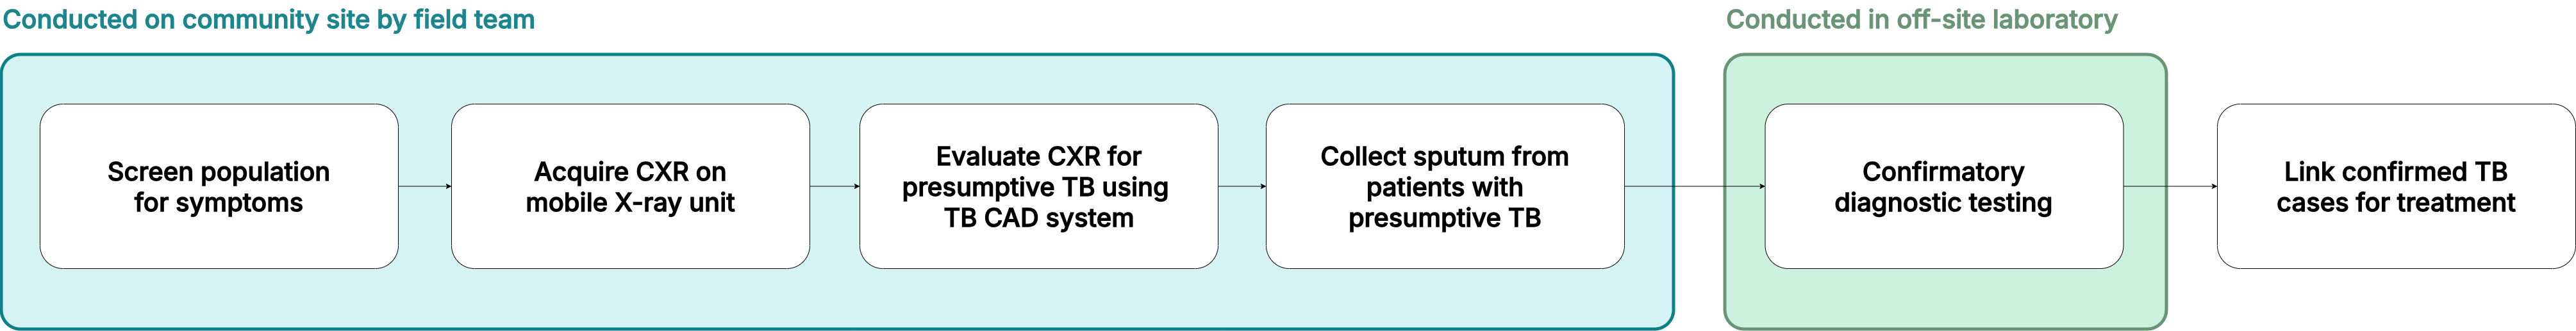
\includegraphics[width=\textwidth]{../figures/ACF Workflow.png}
    \caption{A sample community-based ACF workflow for TB screening. The CAD system in ACF is often used by a radiographer rather than a radiologist.}
    \label{fig:acf}
\end{figure*}

\subsection{Challenges in CAD Integration in Community-based ACF}

While TB CAD systems are highly accurate, CAD workflow integration, local validation, and human factors are relatively under-studied~\cite{kallianos2019review, ahmad2023systematic}. ACF, in particular, faces barriers in connectivity, compute, and interpretation:

\textbf{Connectivity and compute are constrained in community sites.} ACF is often conducted in remote sites where connectivity is unstable and CAD software runs on laptops~\cite{stoptb_cad_guide}. Several implementation studies document how these constraints shape field deployment~\cite{stoptb_cad_guide, vijayan2023india_tb_cad, innes2023vietnam_tb_cad}.

\textbf{CAD overlays are designed for radiologist readers, whereas ACF teams often do not have radiologists.} We review the six TB CAD products approved by WHO in 2025~\cite{who_cad_approval_2025}: qXR v4.0~\cite{qxr_docs}, CAD4TB v7~\cite{cad4tb_product}, Lunit INSIGHT CXR v3.1~\cite{lunit_product}, DrAid v2.4.4--6~\cite{draid_product}, Genki Edge v3.4.2~\cite{genki_product}, and InferRead DR Chest v1.0.1.1~\cite{inferread_product}. All products output probability scores for abnormalities with visual localization through bounding boxes, outlines, or heatmaps. However, these are primarily designed for radiologists, rather than for non-radiologist readers in ACF settings. WHO further notes that the average reader in resource-limited settings is likely less proficient than the expert radiologists in CAD evaluation~\cite{who_cad_approval_2025}. Despite CXR interpretation falling outside the radiographer's scope of practice, the radiographer in ACF decides whether to refer a patient for confirmatory testing using the patient's symptoms and the CAD output~\cite{find_cad_landscape, stoptb_cad_guide}. CAD overlays also overlap poorly with expert-identified regions and omit the contextual reasoning used in diagnosis~\cite{chen2022xai_human_centered}, hence textual descriptions have been proposed as a clinically meaningful complement to CAD overlays~\cite{hua2025qxr_acceptability, ihongbe2024xai_cxr, borys2023xai_beyond_saliency, siemens_llm_cxr_2023, gaube2024care_explain}.

\subsection{Related Work}

TB CAD models with lightweight memory and compute have been explored in previous studies, from LightTBNet at about 1.5M parameters~\cite{capellan2023lighttbnet} to lightweight hybrid networks~\cite{owda2025hybrid_tb}, building on edge-deployed CXR models for related conditions~\cite{benmalek2025edge, chauhan2024covid_edge}. Due to compute constraints in ACF, some existing commercial CAD systems require a dedicated CAD box or separate CAD laptop to support offline screening~\cite{stoptb_cad_guide}.

Related literature has also explored models that generate natural-language descriptions of findings. In a research prototype, Siemens Healthineers paired a combined classification-localization model~\cite{ghesu2022ssl_medical} with a domain-adapted LLM to generate CXR findings~\cite{siemens_llm_cxr_2023}. General medical vision-language models such as LLaVA-Med~\cite{li2023llava_med} and CXR-LLaVA~\cite{lee2024cxr_llava} demonstrate image-conditioned radiology text generation~\cite{bazi2024vlm_review}. However, prior work remains in general chest X-ray detection, with few known to be specific to TB. Of the few TB-specific studies, generative models are used~\cite{ganapthy2025tb_vlm} that carry hallucination risk and heavier inference than a screening pipeline that must run offline on a commodity CPU.

Prior TB CAD systems validated for ACF and non-radiologist screening, such as CAD4TB~\cite{cad4tb_product}, qXR~\cite{qxr_docs}, and Lunit INSIGHT CXR~\cite{lunit_product}, are closed-source commercial products with per-study license and imaging-hardware costs and output specific radiographic findings for radiologist readers. To our knowledge, no prior work develops an open-source TB CAD pipeline that runs offline on a laptop CPU with report generation designed primarily for non-radiologist readers.

\subsection{Contributions}

This study presents a lightweight TB screening pipeline for community ACF where there is no on-site radiologist, no GPU, and unreliable connectivity. We present the following:

\begin{itemize}
    \item A screening pipeline that runs offline on a commodity laptop CPU, completing a study in about 370 ms for community ACF constraints.
    \item A template-based natural-language report for non-radiologist ACF readers to base referral decisions.
    \item Open-sourced TB CAD pipeline as a cheaper alternative to per-study licensing and hardware costs of commercial systems.
    \item Evaluation of four detectors for both computational cost and detection of active \& latent TB, where latent TB is underdetected in prior work.
    \item Evaluation of ten classifiers against WHO TB CAD targets, measured in-distribution on TBX11K and out-of-distribution on Montgomery and Shenzhen datasets.
\end{itemize}

% ============================================================
% II. MATERIALS AND METHODS
% ============================================================
\section{System Overview}

\begin{figure}[!t]
    \centering
    \includegraphics[width=\linewidth]{../figures/pipeline.png}
    \caption{Overview of the TB CAD pipeline.}
    \label{fig:pipeline}
\end{figure}

An overview of the TB CAD pipeline is shown in Figure \ref{fig:pipeline}. A CXR (in DICOM or standard image format) is ingested from the screening unit's X-ray or uploaded directly, then scored by the TB classification module. For images flagged as TB, the object detection module identifies active and latent TB regions. The classification and detection outputs are passed to the report generation module, which outputs a natural-language report of the detected TB regions in a format similar to radiologic convention. Report findings consist of active TB and latent TB lesions rather than specific radiographic findings typical to radiologic reports because the report is designed for non-radiologist readers. All three stages are lightweight for ACF screening where no radiologist and often no GPU is present.

% ============================================================
% TUBERCULOSIS CLASSIFICATION
% ============================================================
\section{Tuberculosis Classification}
\label{sec:tb_classification}

The TB classification module flags each CXR as either healthy, sick non-TB, or TB as shown in Figure~\ref{fig:pipeline}.

\subsection{Dataset}

Classification and object detection models are trained on a simplified redistribution\footnote{\url{https://www.kaggle.com/datasets/vbookshelf/tbx11k-simplified}} of TBX11K~\cite{liu2020tbx11k}, a public CXR dataset with image-level labels (\textit{healthy}, \textit{sick non-TB}, \textit{TB}) and bounding-box-level labels (\textit{active-TB}, \textit{latent-TB}).

TBX11K is selected because it is the largest public TB CXR dataset with a TB-specific sample large enough to train from scratch, expert bounding-box annotations, a sick non-TB class, and a demographic and class composition that reflect real-world clinical settings~\cite{liu2023tbx11k_pami}. Its image-level labels are established by diagnostic microbiology~\cite{liu2023tbx11k_pami}, the reference standard for TB confirmation~\cite{liu2023tbx11k_pami, who_cad_approval_2025}. TBX11K is composed mostly of TB cases aged 20-60, predominantly among males (72\% of TB X-rays), which is representative of real-world TB distribution~\cite{liu2023tbx11k_pami}.

The official TBX11K test set is withheld for an online challenge, so we use only the public trainval images. Our results are therefore not directly comparable to SymFormer~\cite{liu2023tbx11k_pami} or other challenge entries on the private test set. The data used is made available in the Data and Code Availability section of this study.

\begin{table}[!ht]
\renewcommand{\arraystretch}{1.2}
\centering
\begin{threeparttable}
\caption{TBX11K Dataset Composition (Image-level Labels) for Classification}
\label{tab:dataset_composition}
\small
\begin{tabularx}{\columnwidth}{@{}l *{4}{C}@{}}
\toprule
\textbf{Class} & \textbf{Train} & \textbf{Val} & \textbf{Test} & \textbf{Total} \\
\midrule
Healthy        & 2,660 & 570   & 570   & 3,800 \\
Sick non-TB    & 2,660 & 570   & 570   & 3,800 \\
TB             & 560   & 120   & 120   & 800 \\
\midrule
Total          & 5,880 & 1,260 & 1,260 & 8,400 \\
\bottomrule
\end{tabularx}
\end{threeparttable}
\end{table}

Classification uses the image-level labels shown in Table~\ref{tab:dataset_composition}. The 8,400 public CXRs (3,800 healthy, 3,800 sick non-TB, 800 TB) are partitioned per class into train, validation, and test folds in a 70\%/15\%/15\% ratio. All reported classification metrics are computed on the held-out test fold of 1,260 CXRs (570 healthy, 570 sick non-TB, 120 TB).

\subsection{Data Preprocessing}

Classification models are trained without preprocessing or data augmentation. TBX11K CXRs are acquired under a standardized posteroanterior protocol and are largely uniform in pose, so   augmentation risks introducing distribution shift.

\subsection{Model Architecture}

We evaluate ten classifiers: six baselines (EfficientNet-B0~\cite{tan2019efficientnet}, MobileNetV3-Large~\cite{howard2019mobilenetv3}, DenseNet-121~\cite{huang2017densenet}, ResNet-18, ResNet-50~\cite{he2016resnet}, ConvNeXt-Tiny~\cite{liu2022convnext}), three custom models (DraxNet, Drax-MobileNetV3-Large, FlipR), and LightTBNet~\cite{capellan2023lighttbnet}, a published TB-specific lightweight network retrained under our protocol. Full architecture of custom models are listed in Appendix \ref{app:architectures}.

\subsubsection{DraxNet}

DraxNet ($16.5$M parameters) modifies a ResNet-18 backbone so the fourth stage consists of two residual blocks, each with a custom mixer (\emph{DraxBlock}) inserted between its two convolutions. All other components are unchanged. \emph{DraxBlock} consists of a ConvNeXt local convolutional branch followed by an optional self-attention branch, fused via stochastic-depth residuals. DraxNet, short for Dynamic Residual Attention eXchange, reserves the heavier mixer for the final, lowest-resolution stage, adding attention capacity with fewer parameters than a full attention backbone.

\subsubsection{Drax-MobileNetV3-Large}

Drax-MobileNetV3-Large ($4.8$M parameters) applies the DraxBlock to a parameter-efficient backbone. The MobileNetV3-Large feature extractor and head are unchanged, and a bottlenecked \emph{DraxBlock} is inserted after the final feature stage. This design tests whether the DraxBlock generalizes beyond a ResNet-style backbone.

\subsubsection{FlipR}

FlipR ($2.8$M parameters) inserts a \emph{FlipR} block between the second and third stages of a ResNet-18 truncated to three stages, with the parameter-heavy fourth stage removed. The \emph{FlipR} block computes the difference between each feature map and its horizontally flipped counterpart, smoothed by average pooling to account for imperfect anatomical symmetry, then broadcasts a gated mask across all channels. The block is inspired by SymAttention~\cite{liu2023tbx11k_pami}, which observes that bilateral asymmetry in CXRs is a key indicator of TB. FlipR tests whether a lightweight symmetry gate can match heavier attention approaches.

\subsection{Model Training}

All models are trained from scratch with a fixed random seed, batch size $16$, $512\times512$ input, $100$ epochs, Adam optimizer at a fixed learning rate of $10^{-3}$, and unweighted cross-entropy loss. No hyperparameter tuning was done. The checkpoint with the lowest validation loss is retained and evaluated on the held-out test fold.

\subsection{Results}

\begin{table*}[!t]
\renewcommand{\arraystretch}{1.2}
\centering
\begin{threeparttable}
\caption{Tuberculosis Classification Results}
\label{tab:classification_results}
\small
\setlength{\tabcolsep}{2.2pt}
\begin{tabularx}{\textwidth}{@{}l *{10}{C}@{}}
\toprule
\multirow{2}{*}{\textbf{Model}} & \multirow{2}{*}{\textbf{AUC$_{\text{TB}}$}} & \multicolumn{7}{c}{\textbf{Classification metrics (\%)}} & \multicolumn{2}{c}{\textbf{Computational metrics}} \\
\cmidrule(lr){3-9}\cmidrule(lr){10-11}
 & & \textbf{Acc} & \textbf{Sens} & \textbf{Spec} & \textbf{Prec} & \textbf{Rec} & \textbf{F1} & \textbf{\shortstack{Spec@90\\Sens}} & \textbf{Params} & \textbf{MACs} \\
\midrule
LightTBNet~\cite{capellan2023lighttbnet} & 0.9994 & 98.89 & 94.17 & \textbf{99.82} & 98.72 & 97.65 & 98.17 & 99.82 & \textbf{1.3M} & 14.1G \\
FlipR                  & 0.9987 & 98.81 & 94.17 & 99.56 & 98.01 & 97.59 & 97.79 & 99.82 & 2.8M & 7.4G \\
EfficientNet-B0~\cite{tan2019efficientnet} & \textbf{0.9995} & 98.89 & 95.00 & 99.65 & 98.29 & 97.87 & 98.07 & \textbf{100.00} & 4.0M & 2.1G \\
MobileNetV3-Large~\cite{howard2019mobilenetv3} & \textbf{0.9995} & \textbf{99.21} & \textbf{96.67} & \textbf{99.82} & \textbf{98.97} & \textbf{98.54} & \textbf{98.75} & \textbf{100.00} & 4.2M & \textbf{1.2G} \\
Drax-MobileNetV3-Large & 0.9989 & 98.81 & 95.00 & 99.65 & 98.23 & 97.81 & 98.02 & \textbf{100.00} & 4.8M & 1.3G \\
DenseNet-121~\cite{huang2017densenet} & 0.9975 & 98.57 & 92.50 & 99.56 & 97.81 & 96.97 & 97.38 & 99.82 & 7.0M & 15.0G \\
ResNet-18~\cite{he2016resnet} & 0.9982 & 98.17 & 93.33 & 99.21 & 96.71 & 96.90 & 96.80 & 99.91 & 11.2M & 9.5G \\
DraxNet                & 0.9988 & 98.41 & 95.00 & 99.47 & 97.51 & 97.51 & 97.51 & \textbf{100.00} & 16.5M & 10.9G \\
ResNet-50~\cite{he2016resnet} & 0.9978 & 97.70 & 92.50 & 99.47 & 96.95 & 96.33 & 96.63 & 99.47 & 23.5M & 21.5G \\
ConvNeXt-Tiny~\cite{liu2022convnext} & 0.9952 & 97.14 & 95.00 & 97.98 & 93.63 & 96.58 & 94.97 & 99.82 & 27.8M & 23.4G \\
\bottomrule
\end{tabularx}
\begin{tablenotes}[flushleft]
\footnotesize
\item AUC$_{\text{TB}}$ is the area under the ROC curve for the TB class. Sensitivity is recall for the TB class. Specificity is recall for the non-TB class (healthy and sick non-TB combined). Precision, recall, and F1 are averaged across the three classes (healthy, sick non-TB, TB). Params is the trainable parameter count. MACs is the number of multiply-accumulate operations for one forward pass. FLOPs are twice MACs. Spec@90Sens is the specificity when sensitivity is set to $90\%$, which is the operating point calibration used in WHO 2025 evaluation. WHO recommends minimum $40\%$ specificity when fixed at $90\%$ sensitivity~\cite{who_cad_approval_2025}.
\end{tablenotes}
\end{threeparttable}
\end{table*}


Classification results are reported in Table~\ref{tab:classification_results}.

\textbf{No single model is lightest on both storage and compute.} Lighter models show a trade-off between storage use through params and computational cost through MACs. LightTBNet has the fewest parameters ($1.3$M) at the cost of higher MACs ($14.1$G), and models with MobileNet backbones have the fewest MACs ($1.2-1.3$G) at the cost of higher parameters ($4.2-4.8$M). Hence, the model choice depends on whether storage or compute is the tighter constraint in deployment.

\textbf{Bilateral asymmetry is a strong indicator of TB.}
FlipR is the second smallest model by parameters ($2.8$M) and achieves performance within $1\%$ of the top four baselines (LightTBNet, EfficientNet-B0, MobileNetV3-Large, Drax-MobileNetV3-Large) in both accuracy and F1. FlipR's performance despite lighter parameters is consistent with the SymFormer~\cite{liu2023tbx11k_pami} observation that bilateral asymmetry is a strong indicator of TB. Its parameter savings come from removing the parameter-heavy final stage of ResNet-18, which runs at low resolution and thus contributes little compute. FlipR roughly halves LightTBNet's compute ($7.4$G) but still exceeds the MobileNet backbones (MobileNetV3-Large $1.2$G, Drax-MobileNetV3-Large $1.3$G).

\textbf{All models exceed WHO 2025 TB CAD targets on the TBX11K test set, but likely reflects lower task difficulty compared to the WHO test set.}
In the 2025 WHO TB CAD evaluation, two conditions are evaluated: 1.) specificity must meet a minimum of $40\%$ when sensitivity is fixed to $90\%$, and 2.) partial AUC over the $40$ to $60\%$ specificity range is evaluated~\cite{who_cad_approval_2025}. All models exceed the minimum specificity target as shown in Table \ref{tab:classification_results} and achieve a perfect partial AUC of $1.00$ over the $40$ to $60\%$ specificity range. However, WHO selected $40\%$ specificity as this is close to expert radiologist performance on WHO's private test set, not on the TBX11K test set, hence results are indicative but not directly comparable. The WHO test set is presumed to be more difficult than the TBX11K test set. Although both are labelled based on microbiological reference standard, TBX11K is single-demographic and curated from facility screening CXRs, whereas the WHO test set is from multiple demographics with CXRs specifically from community screening. Because no known public TB dataset matches this, evaluating the classifiers on a comparable multi-demographic dataset against radiologist performance remains future work.

\textbf{The high-specificity, lower-sensitivity profile is likely attributable to TBX11K rather than model architecture.}
All models display high specificity and lower sensitivity, consistent with results from models in related literature trained on TBX11K. Sensitivity is more clinically important than specificity in screening, because a missed TB case risks untreated transmission while a false positive triggers only unnecessary confirmatory testing. The TBX11K dataset is constructed to reward high specificity because the common failure mode on other TB datasets is over-predicting TB and achieving near-zero specificity. This is consistent with the performance of other models on the TBX11K dataset~\cite{liu2023tbx11k_pami}.

\textbf{Lightweight models are preferred for TB screening on both performance and deployment grounds.}
The smaller models (LightTBNet, FlipR, EfficientNet-B0, MobileNetV3-Large, Drax-MobileNetV3-Large) match or exceed every larger model in accuracy and F1. Due to a modest TBX11K training set, a minority TB class, and no class-imbalance handling, we hypothesize that this is because larger networks overfit the majority healthy and sick non-TB classes rather than learn discriminative TB features. Due to compute constraints in ACF, lightweight models are preferred for both performance and practical deployment.

\subsection{Out-of-distribution Validation}
\label{subsec:external_validation}

\begin{table*}[!t]
\renewcommand{\arraystretch}{1.2}
\centering
\begin{threeparttable}
\caption{AUC$_{\text{TB}}$ of Models on Out-of-Distribution Datasets}
\label{tab:external_validation}
\small
\begin{tabular}{@{}l c ccc ccc@{}}
\toprule
 & & \multicolumn{3}{c}{\textbf{Montgomery}} & \multicolumn{3}{c}{\textbf{Shenzhen}} \\
\cmidrule(lr){3-5}\cmidrule(lr){6-8}
\textbf{Model} & \textbf{In-dist} & \textbf{Zero-shot} & \textbf{AdaBN} & \textbf{Crop} & \textbf{Zero-shot} & \textbf{AdaBN} & \textbf{Crop} \\
\midrule
LightTBNet~\cite{capellan2023lighttbnet} & 0.999 & 0.470 & \textbf{0.571} & 0.432 & 0.394 & 0.375          & \textbf{0.430} \\
FlipR                  & 0.999 & \textbf{0.669} & 0.618          & 0.645 & 0.688 & 0.676          & \textbf{0.705} \\
EfficientNet-B0~\cite{tan2019efficientnet} & 0.999 & 0.466 & \textbf{0.602} & 0.551 & 0.614 & 0.463          & \textbf{0.717} \\
MobileNetV3-Large~\cite{howard2019mobilenetv3} & 0.999 & 0.426 & \textbf{0.589} & 0.260 & 0.511 & 0.326          & \textbf{0.688} \\
Drax-MobileNetV3-Large & 0.999 & 0.571 & \textbf{0.725} & 0.384 & 0.475 & 0.434          & \textbf{0.569} \\
DenseNet-121~\cite{huang2017densenet} & 0.997 & 0.511 & 0.537          & \textbf{0.552} & 0.495 & 0.545 & \textbf{0.594} \\
ResNet-18~\cite{he2016resnet} & 0.998 & \textbf{0.613} & 0.610 & 0.568 & 0.639 & 0.565          & \textbf{0.727} \\
DraxNet                & 0.999 & 0.563 & 0.591          & \textbf{0.599} & 0.604 & 0.599 & \textbf{0.754} \\
ResNet-50~\cite{he2016resnet} & 0.998 & \textbf{0.636} & 0.625 & 0.635 & 0.637 & 0.612          & \textbf{0.785} \\
ConvNeXt-Tiny~\cite{liu2022convnext} & 0.995 & \textbf{0.697} & --    & 0.599 & 0.613 & --             & \textbf{0.687} \\
\midrule
Mean                   & 0.998 & 0.562 &                &       & 0.567 &                &                \\
\bottomrule
\end{tabular}
\begin{tablenotes}[flushleft]
\footnotesize
\item Each trained classifier is evaluated, without retraining, on the Montgomery and Shenzhen sets~\cite{jaeger2014datasets}, scoring TB triage as binary with $P(\text{TB})$ as the positive score and healthy and sick non-TB pooled as negative. \textbf{In-dist} is the within-TBX11K AUC$_{\text{TB}}$ from Table~\ref{tab:classification_results}. \textbf{Zero-shot} applies the model as trained. \textbf{AdaBN} recomputes batch-normalization statistics on the unlabeled target images. AdaBN is not applicable to ConvNeXt-Tiny, which uses layer normalization rather than batch normalization. \textbf{Crop} restricts the input to the segmented lung field. Bold marks the best correction (among zero-shot, AdaBN, and crop) per model and dataset.
\end{tablenotes}
\end{threeparttable}
\end{table*}

To test out-of-distribution performance, we run each classifier without retraining on two public CXR sets from different countries and scanners: the Montgomery County set (138 images, 58 TB) and the Shenzhen set (662 images, 336 TB)~\cite{jaeger2014datasets}. Results are reported in Table~\ref{tab:external_validation}.

\textbf{Zero-shot performance on out-of-distribution data collapses from near-perfect to weak.}
Both Montgomery and Shenzhen datasets are binary classification tasks, hence performance is evaluated with no TB and sick non-TB labels from TBX11K as the negative class and TB as the positive class. Mean AUC$_{\text{TB}}$ for all models falls from $0.998$ within TBX11K to $0.564$ across the two external sets, with several models at or below chance. Figure~\ref{fig:ood_roc} shows this collapse for the deployed FlipR classifier. The saturated in-distribution figures therefore reflect a single curated source rather than transferable screening skill. Models should be trained on a more diverse dataset in future work and calibrated per community site as per WHO guidance~\cite{who_cad_approval_2025}.

\begin{figure}[!t]
    \centering
    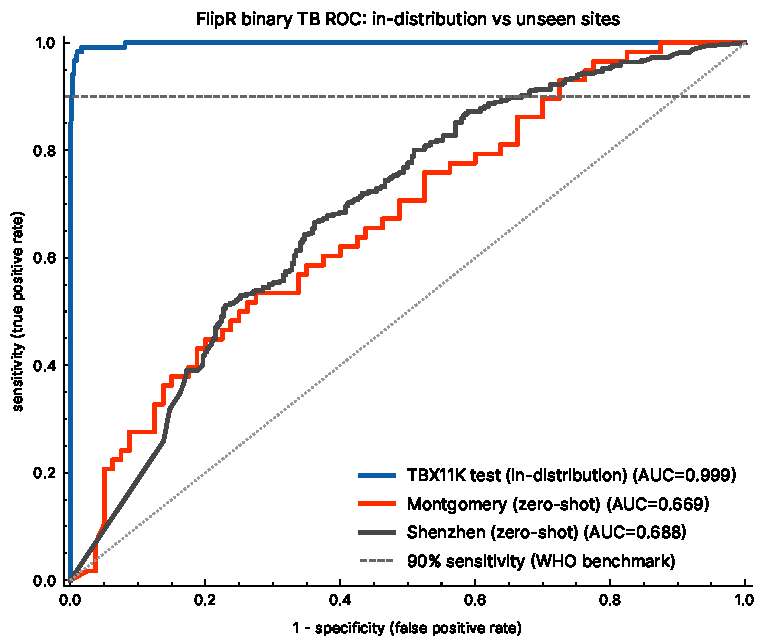
\includegraphics[width=\linewidth]{../figures/classifier_ood_roc/classifier_ood_roc.pdf}
    \caption{Binary TB ROC for the FlipR classifier on the in-distribution TBX11K test set against the two unseen sites, Montgomery and Shenzhen. The in-distribution curve saturates in the top-left corner while both external curves fall toward the diagonal, showing the AUC collapse reported in Table~\ref{tab:external_validation}. The dashed line marks the $90\%$ sensitivity operating point from WHO 2025 targets (minimum $40\%$ specificity at $90\%$ sensitivty)~\cite{who_cad_approval_2025}.}
    \label{fig:ood_roc}
\end{figure}

\textbf{Model performance on the two sets fail in opposite directions due to shifts in image appearance across sets.}
On Montgomery the models lose sensitivity, under-flagging TB images, while on Shenzhen the models lose specificity, over-flagging normal images. The two sets differ from the TBX11K training images in opposite ways in mean pixel intensity (Montgomery is darker at $113$, Shenzhen is brighter at $157$, compared to $123$ for TBX11K), with a Jensen-Shannon divergence of intensity histograms from the training set of $0.30$ and $0.29$ respectively (Figure~\ref{fig:domain_gap}). Because the direction of failure on each set is consistent with this, the collapse is likely due to a shift in image appearance rather than an artifact of adapting the three-class model to binary.

\textbf{Two corrections recover model performance without retraining.}
Real ACF CAD deployment should adapt to a new community site without relabeling, so we test two standard corrections that use only the unlabeled target images and leave all learned weights fixed. Adaptive batch normalization (AdaBN) recomputes each batch-normalization layer's running statistics on the target images~\cite{li2018adabn}. Lung-field cropping restricts the input to the lungs using an off-the-shelf segmentation model~\cite{cohen2022torchxrayvision}, removing burned-in text, borders, and field-of-view differences that are known cross-dataset shortcuts~\cite{zech2018shortcut}. The two corrections address different shift components. AdaBN recovers Montgomery, the intensity-shifted set, raising MobileNetV3-Large from $0.426$ to $0.589$ and Drax-MobileNetV3-Large from $0.571$ to $0.725$, whereas cropping recovers Shenzhen, the framing-shifted set, raising ResNet-50 from $0.637$ to $0.785$ and DraxNet from $0.604$ to $0.754$. Neither correction helps both datasets, consistent with each addressing a distinct difference in each dataset from training data. Across the ten models, applying the better correction per set raises mean AUC$_{\text{TB}}$ from $0.544$ to $0.643$, with the strongest models reaching $0.72$ to $0.79$. However, these figures remain below the in-distribution values and below the WHO operating targets, and thus do not establish deployment readiness. The results show instead that performance collapse is likely due to need for site calibration, which is correctable and consistent with WHO's guidance to calibrate TB CAD systems per community site~\cite{who_cad_approval_2025}, rather than due to a loss of learned TB features.

% ============================================================
% TUBERCULOSIS LESION DETECTION
% ============================================================
\section{Tuberculosis Lesion Detection}
\label{sec:tb_localization}

The object detection module localizes each abnormality on the CXR with a bounding box and classifies each abnormality as either an active TB or latent TB lesion.

\subsection{Dataset}

\begin{table}[!ht]
\renewcommand{\arraystretch}{1.2}
\centering
\begin{threeparttable}
\caption{TBX11K Dataset Composition (Bounding Box Labels) for Lesion Detection}
\label{tab:localization_composition}
\small
\begin{tabularx}{\columnwidth}{@{}l *{3}{C}@{}}
\toprule
\textbf{Annotation} & \textbf{Train} & \textbf{Test} & \textbf{Total} \\
\midrule
Active-TB boxes & 724 & 248 & 972 \\
Latent-TB boxes & 178 & 61 & 239 \\
\midrule
Total boxes & 902 & 309 & 1,211 \\
\bottomrule
\end{tabularx}
\begin{tablenotes}[flushleft]
\footnotesize
\item Counts of bounding boxes. The 800 TBX11K images classified as TB on the image-level label contain 1,211 boxes because one image may have multiple boxes.
\end{tablenotes}
\end{threeparttable}
\end{table}

Object detection uses the TBX11K bounding-box annotations, with each region labeled active TB or latent TB. Dataset composition is shown in Table \ref{tab:localization_composition}.

Active TB denotes ongoing, transmissible infection requiring treatment. Latent TB denotes prior, inactive infection including healed lesions that are not contagious but may reactivate. As Figure~\ref{fig:pipeline} shows, active TB is more visually salient and latent TB is more subtle. A CXR with an image-level label of TB may contain bounding box labels of only active-TB lesions ($630$ images), only latent-TB lesions ($139$ images), or both ($30$ images). This composition is consistent with real-world conditions, where active TB is more common than latent TB~\cite{liu2020tbx11k}.

Differentiation between active and latent TB is relatively understudied in TB CAD. In routine reporting, a radiologist may not always state whether a lesion is suspected as active or latent TB explicitly, instead inferring it from radiographic pattern, with consolidation and cavitation suggesting active disease and fibrotic linear opacities suggesting healed disease, alongside clinical and laboratory correlation~\cite{burrill2007tb_radiology}. Current literature understudies whether existing commercial CAD systems can differentiate latent from active TB~\cite{stoptb_cad_guide}.

\subsection{Model Architecture}

We evaluate four detectors at $256\times256$px input: base YOLO26-n~\cite{yolo26}, two standard nano baselines YOLOv8n~\cite{yolov8} and YOLO11n~\cite{yolo11}, and a custom variant in which YOLO26's default feature extractor is replaced by the DraxNet backbone used in classification. All detectors are trained from random initialization under the same detection head and training protocol. The DraxNet variant retains YOLO26's head, which isolates the backbone's effect relative to base YOLO26.

\subsection{Model Training}

Object detection follows the classification setup in training all detectors from random initialization for $100$ epochs at batch size $16$, but uses the Ultralytics default detection optimizer (auto-selected, base learning rate $10^{-2}$) rather than the Adam optimizer at learning rate $10^{-3}$ used for classification. The best checkpoint (selected by mAP) is retained and used for evaluation.

\subsection{Results}

\begin{table*}[!t]
\renewcommand{\arraystretch}{1.2}
\centering
\begin{threeparttable}
\caption{Tuberculosis Lesion Detection Results}
\label{tab:detection_results}
\small
\begin{tabular}{@{}l cc cc r r@{}}
\toprule
\multirow{2}{*}{\textbf{Model}} & \multicolumn{2}{c}{\textbf{Active TB}} & \multicolumn{2}{c}{\textbf{Latent TB}} & \multirow{2}{*}{\textbf{Params}} & \multirow{2}{*}{\textbf{MACs}} \\
\cmidrule(lr){2-3}\cmidrule(lr){4-5}
 & \textbf{$\mathrm{mAP}_{50}$} & \textbf{$\mathrm{mAP}_{50\text{-}95}$} & \textbf{$\mathrm{mAP}_{50}$} & \textbf{$\mathrm{mAP}_{50\text{-}95}$} & & \\
\midrule
YOLO26~\cite{yolo26} & 0.4511 & 0.2110 & 0.1070 & 0.0410 & \textbf{2.6M} & \textbf{0.5G} \\
YOLO11n~\cite{yolo11} & 0.5434 & 0.2446 & 0.1166 & 0.0435 & \textbf{2.6M} & \textbf{0.5G} \\
YOLOv8n~\cite{yolov8} & 0.5563 & 0.2582 & \textbf{0.1175} & \textbf{0.0444} & 3.2M & 0.7G \\
YOLO26 + DraxNet & \textbf{0.5865} & \textbf{0.2748} & 0.1017 & 0.0310 & 19.7M & 3.2G \\
\bottomrule
\end{tabular}
\begin{tablenotes}[flushleft]
\footnotesize
\item MACs is the number of multiply-accumulate operations for one $256\times256$px forward pass. FLOPs are twice MACs.
\end{tablenotes}
\end{threeparttable}
\end{table*}

Detection results are reported in Table~\ref{tab:detection_results}.

\textbf{Active TB is more likely to be detected than latent TB.}
All detectors localize active TB several times more accurately than latent TB (roughly $3\text{-}6\times$ more accurate for active TB at $\mathrm{mAP}_{50}$ and $3\text{-}9\times$ more accurate at $\mathrm{mAP}_{50\text{-}95}$). This gap reflects the TBX11K class imbalance (active-TB regions outnumber latent-TB regions roughly 4:1) and the subtle appearance of latent-TB lesions. TBX11K also reports the same pattern across all detection methods, attributing it to class imbalance~\cite{liu2023tbx11k_pami}. This pattern is also consistent with radiologist reader performance, where experts distinguish latent TB less reliably than active TB~\cite{choi2023tb_activity}. The bias toward active TB aligns with clinical triage priorities, because active TB requires urgent treatment.

\textbf{The DraxNet backbone improves active-TB localization, but by too small a margin to justify its cost.}
YOLO26 with the DraxNet backbone attains the best active-TB localization at $0.5865$ $\mathrm{mAP}_{50}$ and $0.2748$ $\mathrm{mAP}_{50\text{-}95}$, ahead of the stock YOLOv8n ($0.5563$ and $0.2582$) and YOLO11n ($0.5434$ and $0.2446$). This performance gain comes from replacing base YOLO26's feature extractor: DraxNet raises active-TB $\mathrm{mAP}_{50}$ from $0.4511$ to $0.5865$ ($+0.1354$) and $\mathrm{mAP}_{50\text{-}95}$ from $0.2110$ to $0.2748$ ($+0.0638$) over the base YOLO26, driven almost entirely by precision ($0.74 \rightarrow 0.82$) at unchanged recall (roughly $0.26$). The improvement does not extend to latent TB, where DraxNet is the weakest of the four ($0.1017$ $\mathrm{mAP}_{50}$ against $0.1175$ for YOLOv8n). However, DraxNet's improvement over YOLOv8n is small, about $0.03$ $\mathrm{mAP}_{50}$, while its computational cost is large. The DraxNet backbone uses $19.7$M parameters compared to YOLOv8n's $3.2$M. The marginal active-TB gain does not justify roughly six times the parameters and compute, so we adopt YOLOv8n as the detection model, which is the strongest of the lightweight detectors and within $0.03$ $\mathrm{mAP}_{50}$ of the DraxNet backbone's performance at a fraction of the computational cost.

\begin{figure*}[!t]
\centering
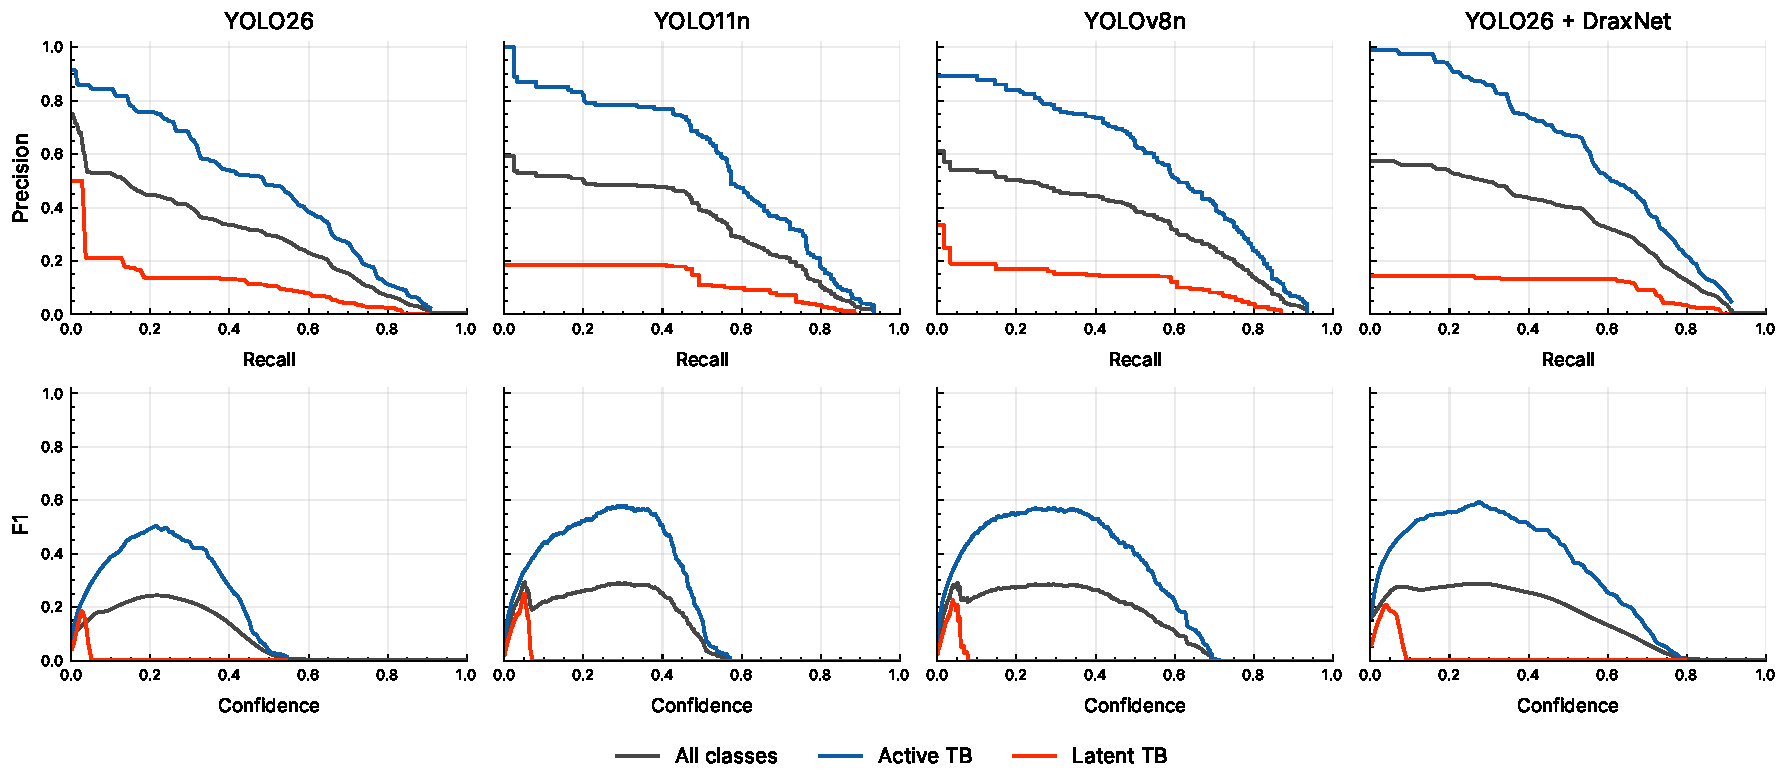
\includegraphics[width=0.98\textwidth]{../figures/detection_curves.pdf}
\caption{Detection precision-recall (top) and F1-confidence (bottom) curves for the four detectors.}
\label{fig:detection_curves}
\end{figure*}

\textbf{Recall, not precision, is the bottleneck.}
Precision stays high while recall lags behind for every detector, so the detectors tend to localize detected TB correctly but miss many TB regions. Figure~\ref{fig:detection_curves} shows recall sits well below precision and the latent-TB curve collapses at low confidence. The pattern is uniform across detectors. Aggregate recall stays near $0.26\text{-}0.28$ for all four models, so no detector flags a substantial fraction of the lesions.

\textbf{Localization is useful to confirm (rule-in) TB, but not to rule it out.} A test rules in disease when a positive result confirms it (rule-in diagnosis) and rules out disease when a negative result excludes it (rule-out diagnosis). The high-precision, low-recall profile indicates that a flagged lesion is likely correct and warrants radiologist review, but the model cannot reliably exclude TB because most annotated lesions are missed. Localization is therefore most reliable as supporting region-level evidence for the classifier and report generation modules, rather than as a standalone detector for TB. Clinicians using the model may reliably use it for rule-in diagnosis, not for rule-out diagnosis.

% ============================================================
% REPORT GENERATION
% ============================================================
\section{Report Generation}
\label{sec:explanation}

The report generation module creates a report for non-radiologist readers to base referral decisions upon. In ACF the reader is a non-radiologist (often a radiographer), so the report is intended to indicate only active or latent TB, rather than full radiographic findings (ex. pleural effusions, cavitations) which are conventional for radiology reports but less intuitive for non-radiologist readers. Example outputs are shown in Figure~\ref{fig:explanation_gallery}.

\begin{figure*}[!t]
\centering
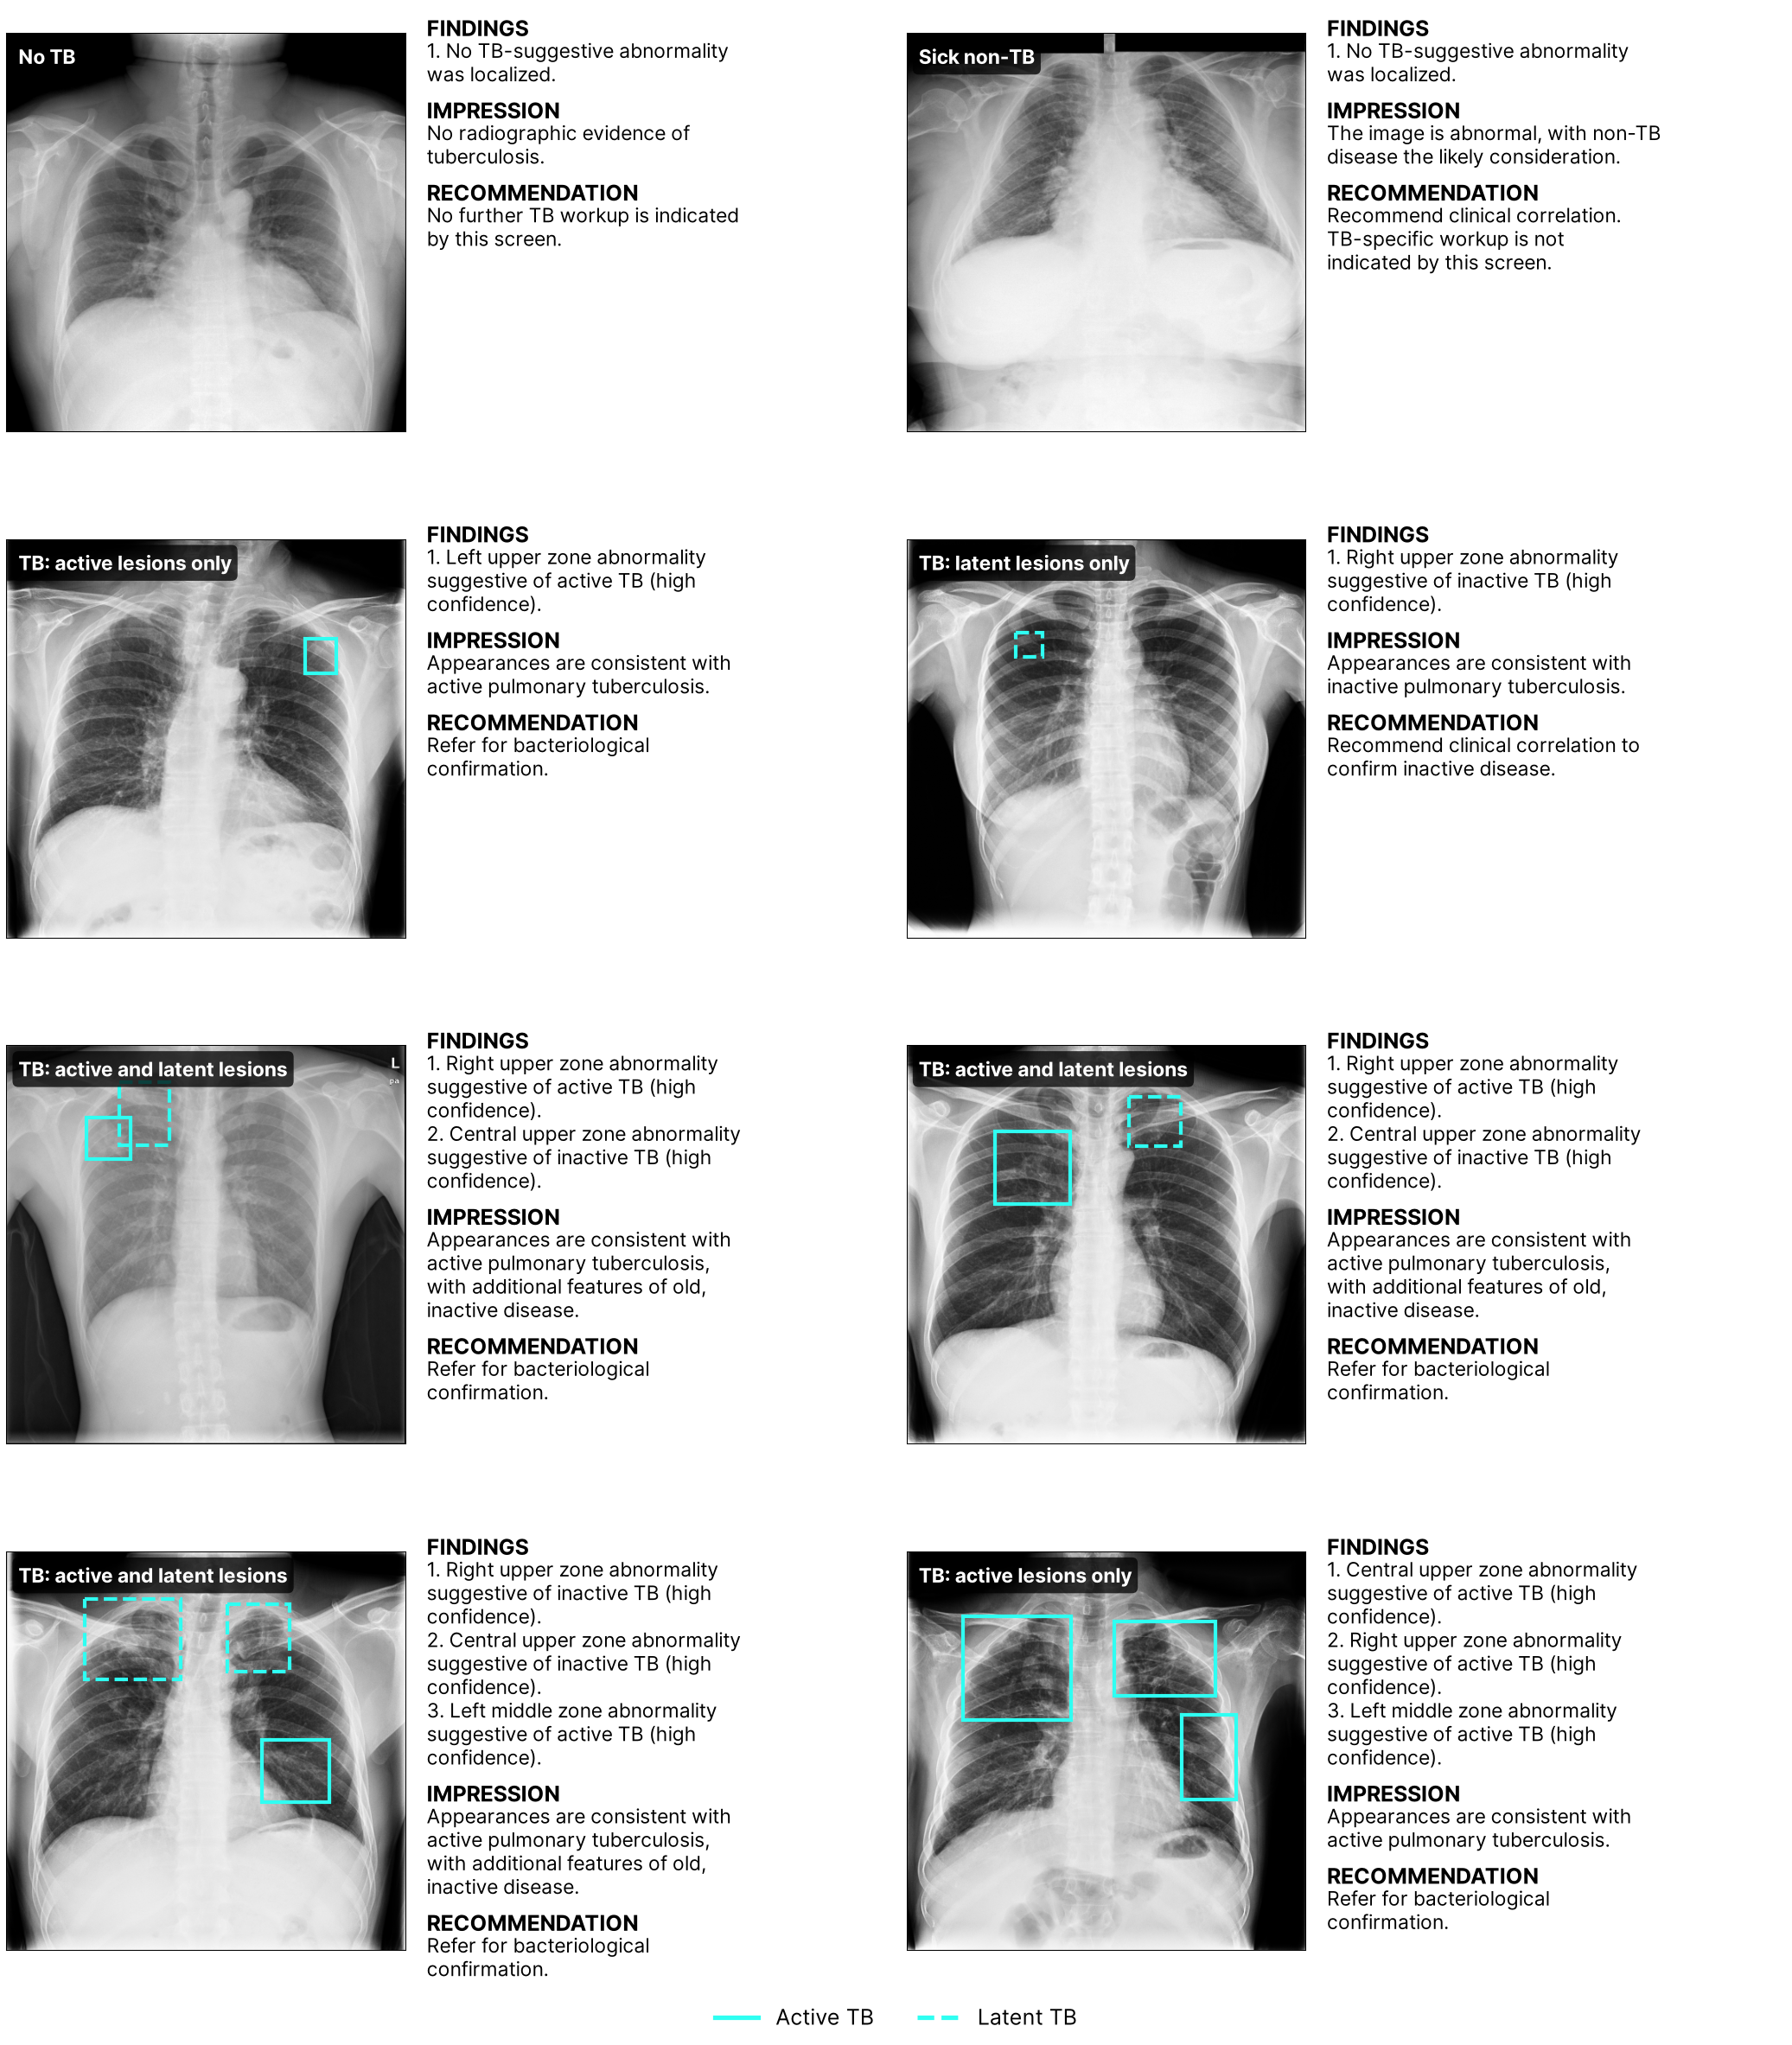
\includegraphics[width=\textwidth]{../figures/cxr_report_gallery/cxr_report_gallery.png}
\caption{Examples of generated reports. The ground-truth class is overlaid at the top-left of each CXR.}
\label{fig:explanation_gallery}
\end{figure*}

This module follows the two-stage detector-to-text architecture of Danu et al.~\cite{siemens_llm_cxr_2023}. However, because our detector emits a closed TB vocabulary rather than open findings, we replace their proprietary detector and fine-tuned language model with the public models of this paper and template-based report generation. Use of a generative model is reserved for future work that detects specific radiographic findings. For current use, template-based report generation suffices and does not require significant memory or compute for resource-constrained ACF settings.

The module has two stages: an adapter that converts raw detector output into a validated structured record, and a template-based report generator that renders that record as text. The second stage receives only a structured record of what the classification and object detection modules produced. This restriction prioritizes faithfulness to model findings, because image-conditioned vision-language models such as CXR-LLaVA~\cite{lee2024cxr_llava} and LLaVA-Med~\cite{li2023llava_med}, as well as related work using LLMs~\cite{siemens_llm_cxr_2023}, may report findings the detector never flagged.

\subsection{Structured Adapter}

The adapter maps classification and detection output to a fixed schema with a small, closed vocabulary. The image-level field carries the predicted label, the argmax over \textit{healthy}, \textit{sick non-TB}, and \textit{TB}, together with its class probabilities. Each detected region carries three fields: its type (\textit{active TB} or \textit{latent TB}), a confidence band (\textit{low}, \textit{medium}, or \textit{high}, thresholded at $0.5$ and $0.8$ on the detection score), and a location. The location is assigned by mapping the bounding-box centroid to one of nine cells in a $3\times3$ grid over the image (upper, middle, or lower row by left, center, or right column). An image with no detections yields an empty region list. The schema is validated before generation, so the report generator always receives well-formed input drawn from this vocabulary. The record states the type and coarse location of each region but no finer radiographic finding, because the detector labels regions only as active or latent TB.

All images are posteroanterior (PA) frontal scans. Hence, the standard radiological laterality convention is used, wherein the patient's right side appears on the image's left side and vice versa. For example, a lesion in the image's upper left corner is reported as an upper right lesion.

\subsection{Template-Based Report Generation}

Template-based report generation is a structured template over the closed schema. It renders the record as a short report in three labeled sections, mirroring the findings-to-impression structure of a radiology report~\cite{zhang2024llm_impressions}: a numbered \textsc{findings} list with one TB region per line including lesion type, model confidence band, and lesion zone, an \textsc{impression} stating the screening result in clinical wording, and a \textsc{recommendation} based on the predicted class, such as referral for bacteriological confirmation when TB is indicated.

The report describes only the detected TB regions and does not name specific radiographic findings such as consolidation, cavitation, or fibrosis, nor cardiac, pleural, and skeletal observations. This reflects both the scarcity of finding-level TB annotations and the report's intended reader, for whom chest X-ray interpretation falls outside the scope of practice and whose task is triage and referral rather than diagnosis. Naming findings that require radiological training to interpret would not change that referral decision and could mislead, whereas the triage label, the region, and the active-versus-latent distinction that bears on referral urgency are what this reader can act on. Richer findings become useful when a radiologist or downstream clinician enters the loop, which, together with the annotation data they require, we leave to future work.

We chose a template over a generative model after prototyping both. An instruction-tuned language-model report generator (Phi-3.5-mini-instruct~\cite{abdin2024phi3}, run image-blind on the same record) was prototyped alongside this work, but the target is a short, fixed-format report with one line per region, which a template reproduces exactly over the closed vocabulary. The template therefore matches the generative output on faithfulness, readability, and the ordering of findings while removing any possibility of hallucination and the model inference cost, an advantage in the resource-limited settings this pipeline targets. A generative model is needed only for future work when the detector reports a richer, open set of interacting findings.

\subsection{Faithfulness by Design}

Report generation is faithful by design, meaning the generated text asserts nothing not present in the structured record. This is the faithfulness-versus-factuality distinction drawn for abstractive summarization~\cite{maynez2020faithfulness} and data-to-text evaluation~\cite{dhingra2019parent}, under which a generation is faithful if every entity it states is supported by the source, independent of whether the source is itself correct. Faithfulness here is the absence of extrinsic hallucination, content asserted in the report that the models did not produce, and it does not by itself imply factual correctness, which remains bounded by the accuracy of the upstream models.

In previous experiments using Phi-3.5-mini-instruct for report generation, we evaluated the result for faithfulness with a deterministic verifier that parses a report for schema entities and flagging any the record does not contain: region type, location, or laterality absent from the record, a predicted label different from the record's, or an invented probability. The verifier follows an established approach in data-to-text generation, extracting the facts a generation asserts and checking them against the source records~\cite{wiseman2017challenges}, and relates to the slot-error and semantic-accuracy metrics from dialogue generation that count output content not licensed by the input meaning representation~\cite{wen2015sclstm, dusek2020semantic}. However, where those methods train an information-extraction or natural-language-inference model because the target text is open, the closed schema makes an exact deterministic match sufficient. Because the template renders deterministically over a validated closed schema, it cannot assert an entity absent from the record, so faithfulness is a structural property of the template and schema rather than an empirical rate measured over outputs. The schema surface is small and closed, so the template cannot render an entity absent from the record: the two region types, three confidence bands, and nine zones, together with the empty-region case for each class, are exhaustively determined by the schema and exercised by representative report-generation tests. Since the generative approach does not provide additional benefit over the template, the generative model is dropped to avoid hallucination risk and reduce compute.

% ============================================================
% DISCUSSION
% ============================================================
\section{On-Device Deployment}

\subsection{Feasibility}

Laptops are typically used to run CAD systems in community-based ACF, resulting in limited compute. CAD is also increasingly deployed offline where network connectivity is unreliable or absent~\cite{stoptb_ultraportable, stoptb_cad_guide}. This mode already operates at scale, with more than 430,000 people screened by ultraportable X-ray and CAD between 2021 and 2023~\cite{min2025scanned}. Models for community-based ACF must be able to run locally on a CPU, without a dedicated GPU or a network connection.

Our lightweight models fall at the parameter scale shown in related literature to run on this class of hardware. Lightweight chest X-ray networks have been deployed on edge devices and CPUs with low latency, including ResNet-18, MobileNet, and EfficientNet-B0 on an embedded board~\cite{benmalek2025edge} and a compact classifier on edge devices~\cite{chauhan2024covid_edge}, and for TB specifically LightTBNet reports rapid, low-memory prediction designed for embedded use~\cite{capellan2023lighttbnet}. Although LightTBNet carries the fewest parameters of our models ($1.3$M), at the $512\times512$ input its MAC cost ($14.1$G) is exceeded only by the three largest models (Table~\ref{tab:classification_results}), so a small parameter count does not by itself imply low compute. FlipR ($2.8$M parameters), Drax-MobileNetV3-Large ($4.8$M), EfficientNet-B0 ($4.0$M), and MobileNetV3-Large ($4.2$M) are at or below the size of those deployed networks, so they should run on the same devices. Their MAC cost at the $512\times512$ input ranges from $1.2$G for MobileNetV3-Large to $7.4$G for FlipR, so the depthwise-separable backbones carry the smallest compute footprint as well as a small memory footprint, while FlipR trades higher compute for a small parameter count. To test these expectations directly, we benchmarked every model on a CPU-only host. Table~\ref{tab:ondevice} reports the single-image latency, peak memory, and on-disk size.

\begin{table}[!t]
\renewcommand{\arraystretch}{1.2}
\centering
\begin{threeparttable}
\caption{On-Device CPU Benchmark}
\label{tab:ondevice}
\small
\begin{tabular}{@{}l r r r r@{}}
\toprule
\textbf{Model} & \textbf{Size} & \textbf{Lat.\ 1T} & \textbf{Lat.\ 6T} & \textbf{RAM} \\
                & \textbf{(MB)} & \textbf{(ms)} & \textbf{(ms)} & \textbf{(MB)} \\
\midrule
\multicolumn{5}{@{}l}{\textit{Classification}} \\
LightTBNet~\cite{capellan2023lighttbnet} & \textbf{5.1} & 621 & 214 & 800 \\
FlipR                  & 11.2 & 244 & 76 & \textbf{603} \\
EfficientNet-B0~\cite{tan2019efficientnet} & 16.3 & 176 & 100 & 654 \\
MobileNetV3-Large~\cite{howard2019mobilenetv3} & 17.0 & \textbf{89} & 58 & 655 \\
Drax-MobileNetV3-Large & 19.4 & 91 & \textbf{56} & 631 \\
DenseNet-121~\cite{huang2017densenet} & 28.4 & 518 & 259 & 806 \\
ResNet-18~\cite{he2016resnet} & 44.8 & 298 & 91 & 629 \\
DraxNet                & 66.0 & 362 & 114 & 649 \\
ResNet-50~\cite{he2016resnet} & 94.4 & 682 & 241 & 819 \\
ConvNeXt-Tiny~\cite{liu2022convnext} & 111.4 & 683 & 217 & 786 \\
\midrule
\multicolumn{5}{@{}l}{\textit{Detection}} \\
YOLO26~\cite{yolo26} & \textbf{5.4} & \textbf{110} & 68 & 620 \\
YOLO11n~\cite{yolo11} & 5.5 & 120 & 56 & \textbf{608} \\
YOLOv8n~\cite{yolov8} & 6.2 & 124 & \textbf{46} & 610 \\
YOLO26 + DraxNet       & 39.7 & 420 & 152 & 727 \\
\bottomrule
\end{tabular}
\begin{tablenotes}[flushleft]
\footnotesize
\item Measured on one Intel Core i7-8750H CPU under PyTorch with float32 compute, batch $1$, $512\times512$ input, and no GPU. Lat.\ 1T and Lat.\ 6T are the median single-image forward-pass latency at $1$ and $6$ CPU threads over $40$ runs. Size is the committed checkpoint on disk. The classification checkpoints store float32 weights, while the Ultralytics detection checkpoints store float16 weights, so detection sizes are about half of (parameters $\times$ $4$ bytes). RAM is the peak resident memory of the whole inference process, which includes a fixed runtime of about $330$ MB ($360$ MB with the detection library). These runtime figures are specific to this host and are not comparable across papers. The portable cost measures are the parameters and MACs in Tables~\ref{tab:classification_results} and~\ref{tab:detection_results}.
\end{tablenotes}
\end{threeparttable}
\end{table}

Every classifier completes a forward pass in under $0.7$ seconds on a single thread and under $0.26$ seconds on six threads, and the whole inference process peaks below $0.82$ GB of memory, so the pipeline runs on a commodity laptop CPU without a GPU. The deployed configuration, FlipR followed by the YOLOv8n detector on a flagged image, runs in about $370$ ms on a single thread and $120$ ms on six threads. On-device latency tracks MACs rather than parameters. The depthwise-separable backbones are fastest, at about $90$ ms on a single thread for MobileNetV3-Large and Drax-MobileNetV3-Large, while FlipR carries few parameters but more compute and takes $244$ ms. LightTBNet makes the point sharply: despite the fewest parameters, its high-resolution design gives it the third-highest single-thread latency at $621$ ms. The FlipR gap narrows to $76$ against $56$ ms at six threads, because FlipR's standard convolutions parallelize across cores better than depthwise convolutions. On-disk size does follow parameter count, where LightTBNet is the smallest at $5.1$ MB and FlipR the next smallest. Peak memory, by contrast, tracks activation size rather than parameters: LightTBNet holds the fewest parameters yet the third-highest peak memory at $800$ MB, because its high-resolution feature maps dominate the footprint. On-disk size therefore follows parameter count, while latency follows MACs and peak memory follows activation resolution.

The detectors show the same pattern. The stock nano detectors localize in $110$ to $124$ ms on a single thread, whereas the DraxNet-backboned variant is about four times slower at $420$ ms and seven times larger on disk, which reinforces the choice of a stock lightweight detector over the DraxNet backbone. These detector latencies are measured at the benchmark's $512\times512$ input, above the $256\times256$ resolution at which the detectors train and deploy, so they are a conservative upper bound on the native-resolution cost. Because latency and peak memory depend on the CPU, the framework, and the thread count, these figures establish feasibility on a commodity CPU rather than on a particular field device, and they are an internally controlled comparison on one host rather than a cross-paper benchmark. A constrained single-board or ARM device would be slower, so characterizing latency on the target deployment hardware remains future work.

\subsection{Cost}

The benchmark above shows that the pipeline runs on a commodity CPU, which also
shapes its cost. We report the compute cost directly, because it follows from the
measured latency, and we place it against published costs for commercial TB CAD
rather than asserting our own figures for products whose prices are not public.

The deployed configuration, FlipR followed by the YOLOv8n detector, completes a
study in about $370$ ms on a single thread (Table~\ref{tab:ondevice}), where the
detector runs only on a flagged image, so this is an upper bound. A screening
program of $100{,}000$ studies per year therefore needs about $10$ CPU-hours of
compute per year. At a commodity cloud CPU rate near $0.045$ USD per core-hour,
that is under $0.50$ USD per year, and on a single $300$ USD offline mini-PC
amortized over a three-year service life, the same workload comes to about $110$
USD per year while leaving the device idle for most of the day. In community active case finding, where the team already
runs CAD on a laptop it owns~\cite{stoptb_cad_guide}, the marginal cost of an
additional study is effectively the electricity, because the pipeline carries no
per-study license.

Commercial TB CAD prices are negotiated and are not published as list
prices~\cite{bashir2022economic}. The firmest public figures are the concessional
bundle prices through the Stop TB Partnership Global Drug Facility, near
$16{,}700$ USD for a perpetual CAD4TB license with hardware, installation, and one
year of support. A multi-product cost model for Pakistan reports per-screen costs
from $0.19$ to $2.73$ USD, where perpetual-license products approach a low
per-screen cost only at high throughput and volume-priced products stay near the
$0.93$ USD cost of a radiologist read~\cite{bashir2022economic}. Field programs
report $13.31$ USD per screen for CAD4TB in Zambia~\cite{jo2021cad4tb} and a
$9{,}000$ USD annual license alongside a $75{,}000$ USD imaging device for qXR in
Nigeria~\cite{garg2025qxr}. These figures use different denominators, base years,
and cost perspectives, so we report them as context rather than as a direct
comparison against the compute cost above.

Across these sources, compute is not the cost driver for TB CAD. Deployment cost
is governed by licensing, imaging hardware, and program logistics. The advantage
of the proposed pipeline is therefore structural rather than a lower unit price
for the same service. It carries no per-study license, runs to completion on a
commodity CPU without a GPU, and adds effectively zero marginal cost per study,
which matters most in the decentralized, low-resource screening settings that the
WHO identifies as the primary setting for automated chest X-ray
interpretation~\cite{who_screening_2021}.

\section{Discussion}

\subsection{Limitations}

TB-specific samples are limited in public datasets. As of writing, TBX11K is the largest public chest X-ray dataset for tuberculosis with labeled bounding boxes, yet its TB subset remains small at 799 TB images and 1,211 TB lesion boxes. While general chest X-ray datasets exist, of these, TB-positive samples are few and insufficient to train from scratch. No public dataset contains TB-specific radiographs with reference radiographic reports, which is what a measurement of clinical correctness would require. This scarcity constrained the development and evaluation of report generation for clinical correctness.

The TB data scarcity limits how representative the evaluation population is. TBX11K is drawn from a single country, from patients presenting for hospital chest examination, and records no HIV status or prior-TB history. The WHO 2025 evaluation instead spans multiple regions, weighted toward high-burden African and South-East Asian settings, and reports lower CAD accuracy among women, people living with HIV, and those with a history of TB~\cite{who_cad_approval_2025}. Reported performance here may therefore overstate what the pipeline would achieve in the higher-burden, HIV-prevalent populations that community active case finding targets. Section~\ref{subsec:external_validation} measures one facet of this gap directly: zero-shot transfer to two other-source sets drops mean AUC$_{\text{TB}}$ from $0.998$ to $0.564$, and although label-free site adaptation recovers part of it, the corrected scores stay below the in-distribution figures. Evaluation on higher-burden, HIV-prevalent populations remains future work.

Although report generation is faithful by design, faithfulness to the detector is not clinical correctness. A report that faithfully restates an incorrect detection is still wrong, and only reference-based or reader evaluation can report this. However, due to the lack of a TB-specific reference dataset, this is left to future work.

The system's scope is limited to screening of non-pediatric patients because the radiographic presentation of pulmonary TB is age-dependent: adult reactivation tuberculosis appears in the upper lung zones, whereas pediatric primary tuberculosis appears in the lower lung zones. Hence, detection patterns learned from a predominantly adult distribution do not transfer to children. This is consistent with the WHO endorsement of CAD as a human-reader alternative only for patients aged 15 years and older~\cite{who_cad_policy_2021}. 

\subsection{Future Work}

Future work seeks to extend the commodity-CPU benchmark reported here (Table~\ref{tab:ondevice}) to the target field hardware, measuring inference latency and memory on constrained single-board or ARM devices under real-world use.

Detection of full radiographic findings, such as cardiac size, pleural fluid, or non-TB abnormalities, as well as cardiac, pleural, and skeletal structures, is reserved for future work given additional data. Specific findings are more clinically meaningful for interpretation of the radiologic report, aligned with human reader interpretation of findings. This would also warrant use of a generative language model over a structured template for report generation, because synthesizing findings into a coherent report is no longer a fixed-format substitution but a genuine generation problem. This is demonstrated by recent chest X-ray systems that aggregate region-level findings into a report with an LLM~\cite{siemens_llm_cxr_2023, noh2026hybrid}.

A reader study with radiologists and non-radiologist screeners is also recommended to evaluate the clinical correctness and coherence of the model-generated reports, particularly in comparison to human reader reports.

% ============================================================
% CONCLUSION
% ============================================================
\section{Conclusion}

TB CAD systems are highly accurate, however challenges remain in integrating them for community ACF with unreliable connectivity, limited compute, and no radiologist present. This paper presented a lightweight TB screening pipeline for that setting. The contribution is the integrated system, not any single model: it pairs lightweight classification and detection with deterministic, faithful-by-design natural-language report generation and runs offline on a commodity laptop CPU, so that instead of a probability score and a heatmap, a non-radiologist reader, in ACF often a radiographer, receives an actionable report built around the triage and referral decision they make rather than the finding-level interpretation a radiologist would perform. The deployed FlipR-and-YOLOv8n configuration completes a study in about 370 ms on this CPU without a GPU. A cost analysis shows that compute is not the cost driver for TB CAD: because the pipeline is open-source it carries no per-study license and adds effectively zero marginal cost per study, so its advantage over commercially available systems is structural rather than a lower unit price. For localization, a comparison of lightweight detectors covers both active and latent TB, the latter underdetected in prior work, and finds that the larger custom DraxNet backbone does not justify its cost, so the compact YOLOv8n detector is preferred for deployment, within a small margin of the best accuracy at a fraction of the footprint, and across all detectors localization functions as a high-precision rule-in cue rather than a standalone detector. Among the classifiers, FlipR achieves similar accuracy and F1 to the strongest baselines with a parameter-efficient design and the best zero-shot transfer to unseen sites. External validation is nonetheless sobering: zero-shot mean TB AUC falls from 0.998 to 0.564 across two unseen sites along a measured intensity shift, and label-free site adaptation recovers only part of the gap while staying below the in-distribution and WHO bars, so the single-source results overstate readiness for multi-site deployment. TB-specific samples were found to be highly limited in public datasets, which constrained the design and evaluation of components. Evaluation rests on a single curated public dataset and on commodity-CPU feasibility, so a full evaluation of deployment feasibility on field hardware, extended radiographic findings for a full radiologist report, and a reader study with radiologists and radiographers in the target populations is left to future work.

% ============================================================
% ACKNOWLEDGMENTS
% ============================================================
\section*{Acknowledgments}

The authors would like to thank the University Research Council (URC) of Ateneo de Manila University for supporting this work through a URC Standard Grant (URC 2025-20). The authors also thank Dr. Reynan B. Hernandez, radiologist at The Medical City and associate professor at the Ateneo School of Medicine and Public Health, for providing medical expertise that informed the clinical grounding of the study.

% ============================================================
% DECLARATION ON GENERATIVE AI
% ============================================================
\section*{Declaration on Generative AI}

Generative AI tools were used to assist in writing the manuscript and source code for the study. All generative AI outputs were reverified by the authors. The conception of the research, methodology, and conclusions are the work of the authors.

% ============================================================
% DATA AND CODE AVAILABILITY
% ============================================================
\section*{Data and Code Availability}

The manuscript, data, and source code for this study is publicly available at \url{https://github.com/alive-ateneo/tb-community-screening-pipeline}.

% ============================================================
% APPENDIX
% ============================================================
\appendices
\section{Architectures of Custom Models}
\label{app:architectures}

\begin{table}[!ht]
\renewcommand{\arraystretch}{1.2}
\centering
\begin{threeparttable}
\caption{FlipR Architecture (ResNet-18 Truncated to Three Stages)}
\label{tab:arch_flipr}
\footnotesize
\begin{tabularx}{\columnwidth}{@{}X c r@{}}
\toprule
\textbf{Stage} & \textbf{Output} & \textbf{Params} \\
\midrule
Stem (conv 7$\times$7, BN, ReLU, pool) & $64\times H/4$ & 9,536 \\
layer1 (2 basic blocks, 64) & $64\times H/4$ & 147,968 \\
layer2 (2 basic blocks, 128) & $128\times H/8$ & 525,568 \\
FlipR gate & $128\times H/8$ & 129 \\
layer3 (2 basic blocks, 256) & $256\times H/16$ & 2,099,712 \\
Head (avg-pool, FC 256$\to$3) & 3 & 771 \\
\midrule
\textbf{Total} & & \textbf{2,783,684} \\
\bottomrule
\end{tabularx}
\end{threeparttable}
\end{table}

\begin{table}[!ht]
\renewcommand{\arraystretch}{1.2}
\centering
\begin{threeparttable}
\caption{DraxNet Architecture (ResNet-18, DraxBlock in Stage 4)}
\label{tab:arch_draxnet}
\footnotesize
\begin{tabularx}{\columnwidth}{@{}X c r@{}}
\toprule
\textbf{Stage} & \textbf{Output} & \textbf{Params} \\
\midrule
Stem (conv 7$\times$7, BN, ReLU, pool) & $64\times H/4$ & 9,536 \\
layer1 (2 basic blocks, 64) & $64\times H/4$ & 147,968 \\
layer2 (2 basic blocks, 128) & $128\times H/8$ & 525,568 \\
layer3 (2 basic blocks, 256) & $256\times H/16$ & 2,099,712 \\
layer4 (2 DraxBlocks, 512) & $512\times H/32$ & 13,699,072 \\
Head (avg-pool, FC 512$\to$3) & 3 & 1,539 \\
\midrule
\textbf{Total} & & \textbf{16,483,395} \\
\bottomrule
\end{tabularx}
\end{threeparttable}
\end{table}

\begin{table}[!ht]
\renewcommand{\arraystretch}{1.2}
\centering
\begin{threeparttable}
\caption{Drax-MobileNetV3-Large Architecture}
\label{tab:arch_draxmobilenet}
\footnotesize
\begin{tabularx}{\columnwidth}{@{}X c r@{}}
\toprule
\textbf{Stage} & \textbf{Output} & \textbf{Params} \\
\midrule
MobileNetV3-Large features & $960\times H/32$ & 2,971,952 \\
DraxBlock adapter (bottleneck 160) & $960\times H/32$ & 575,200 \\
Head (avg-pool, classifier 960$\to$1280$\to$3) & 3 & 1,233,923 \\
\midrule
\textbf{Total} & & \textbf{4,781,075} \\
\bottomrule
\end{tabularx}
\end{threeparttable}
\end{table}

\section{Domain Gap to the External Sites}
\label{app:domain_gap}

\begin{figure}[!ht]
    \centering
    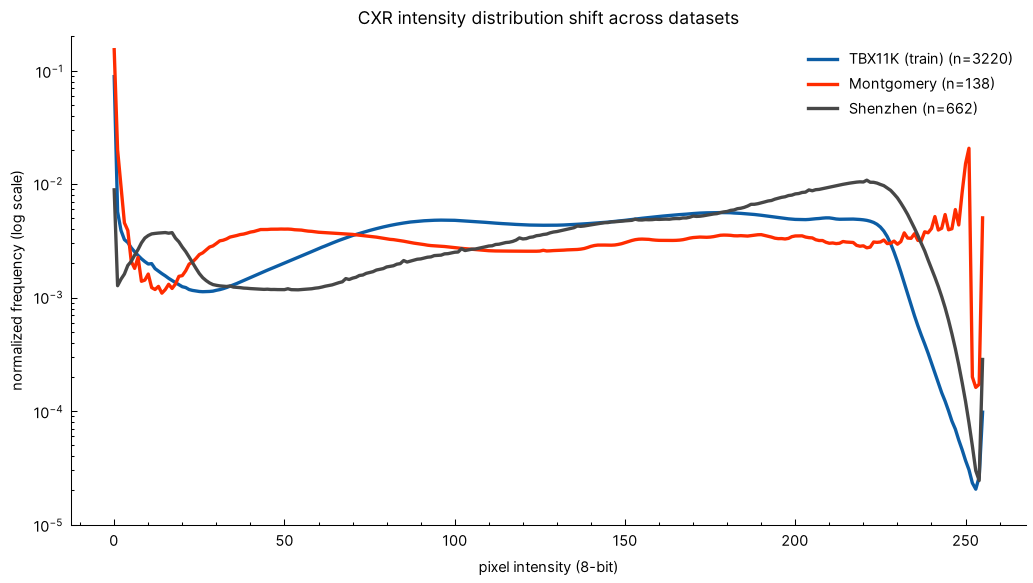
\includegraphics[width=\linewidth]{../figures/domain_gap_hist.png}
    \caption{Pixel-intensity distributions of the TBX11K training images and the two external sites. Montgomery is darker and Shenzhen brighter than the training set, the covariate shift in image appearance discussed in Section~\ref{subsec:external_validation} that tracks the direction of the zero-shot failure on each site.}
    \label{fig:domain_gap}
\end{figure}

% ============================================================
% REFERENCES
% ============================================================
\begin{thebibliography}{40}

\bibitem{who_global_tb_2024}
World Health Organization, ``Global Tuberculosis Report 2024,'' Geneva: WHO, 2024. [Online]. Available: \url{https://www.who.int/teams/global-tuberculosis-programme/tb-reports/global-tuberculosis-report-2024}

\bibitem{who_screening_2021}
World Health Organization, ``WHO consolidated guidelines on tuberculosis. Module 2: Screening -- Systematic screening for tuberculosis disease,'' Geneva: WHO, 2021. [Online]. Available: \url{https://www.who.int/publications/i/item/9789240022676}

\bibitem{pai2016tb}
M. Pai, M. A. Behr, D. Dowdy, K. Dheda, M. Divangahi, C. C. Boehme, A. Ginsberg, S. Swaminathan, M. Spigelman, H. Getahun, D. Menzies, and M. Raviglione, ``Tuberculosis,'' \emph{Nature Reviews Disease Primers}, vol. 2, art. 16076, 2016, doi: 10.1038/nrdp.2016.76.

\bibitem{burrill2007tb_radiology}
J. Burrill, C. J. Williams, G. Bain, G. Conder, A. L. Hine, and R. R. Misra, ``Tuberculosis: A radiologic review,'' \emph{RadioGraphics}, vol. 27, no. 5, pp. 1255--1273, 2007, doi: 10.1148/rg.275065176.

\bibitem{choi2023tb_activity}
Y.~R.~Choi, S.~H.~Yoon, J.~Kim, J.~Y.~Yoo, H.~Kim, and K.~N.~Jin, ``Chest radiography of tuberculosis: determination of activity using deep learning algorithm,'' \textit{Tuberculosis and Respiratory Diseases}, vol.~86, no.~3, pp.~226--233, 2023, doi: 10.4046/trd.2023.0020.

\bibitem{who_cad_policy_2021}
World Health Organization, ``WHO operational handbook on tuberculosis. Module 2: Screening,'' Geneva: WHO, 2021. [Online]. Available: \url{https://www.who.int/publications/i/item/9789240022614}

\bibitem{who_cad_approval_2025}
World Health Organization, ``Use of computer-aided detection software for tuberculosis screening: WHO policy statement,'' Geneva: WHO, 2025. [Online]. Available: \url{https://www.who.int/publications/i/item/9789240110373}

\bibitem{ahmad2023systematic}
H.~K.~Ahmad \textit{et al.}, ``Machine learning augmented interpretation of chest X-rays: A systematic review,'' \textit{Diagnostics}, vol.~13, no.~4, art.~743, 2023. [Online]. Available: \url{https://pmc.ncbi.nlm.nih.gov/articles/PMC9955112/}

\bibitem{anderson2024deep}
P.~G.~Anderson \textit{et al.}, ``Deep learning improves physician accuracy in the comprehensive detection of abnormalities on chest X-rays,'' \textit{Scientific Reports}, vol.~14, 2024. [Online]. Available: \url{https://www.nature.com/articles/s41598-024-76608-2}

\bibitem{kallianos2019review}
K.~Kallianos, J.~Mongan, S.~Antani, T.~Henry, A.~Taylor, J.~Abuya, and M.~Kohli, ``How far have we come? Artificial intelligence for chest radiograph interpretation,'' \textit{Clinical Radiology}, vol.~74, no.~5, pp.~338--345, 2019. [Online]. Available: \url{https://doi.org/10.1016/j.crad.2018.12.015}

\bibitem{siemens_llm_cxr_2023}
M.~D.~Danu, G.~Marica, S.~K.~Karn, B.~Georgescu, A.~Mansoor, F.~Ghesu, L.~M.~Itu, C.~Suciu, S.~Grbic, O.~Farri, and D.~Comaniciu, ``Generation of radiology findings in chest X-ray by leveraging collaborative knowledge,'' \textit{Procedia Computer Science (ITQM 2023)}, 2023. [Online]. Available: \url{https://arxiv.org/abs/2306.10448}

\bibitem{ghesu2022ssl_medical}
F.~C.~Ghesu, B.~Georgescu, A.~Mansoor, Y.~Yoo, D.~Neumann, P.~Patel, R.~S.~Vishwanath, J.~M.~Balter, Y.~Cao, S.~Grbic, and D.~Comaniciu, ``Self-supervised learning from 100 million medical images,'' \textit{arXiv preprint arXiv:2201.01283}, 2022. [Online]. Available: \url{https://arxiv.org/abs/2201.01283}

\bibitem{li2023llava_med}
C.~Li \textit{et al.}, ``LLaVA-Med: Training a large language-and-vision assistant for biomedicine in one day,'' \textit{Advances in Neural Information Processing Systems}, 2023. [Online]. Available: \url{https://arxiv.org/abs/2306.00890}

\bibitem{marquez2025philippines}
N.~Marquez \textit{et al.}, ``Performance of chest X-ray with computer-aided detection powered by deep learning-based artificial intelligence for tuberculosis presumptive identification during case finding in the Philippines,'' \textit{BMC Global and Public Health}, 2025. [Online]. Available: \url{https://bmcglobalpublichealth.biomedcentral.com/articles/10.1186/s44263-025-00198-y}

\bibitem{qxr_docs}
Qure.ai, ``Qure.ai App User's Manual (qXR).'' [Online]. Available: \url{https://documentation.qure.ai/}

\bibitem{cad4tb_product}
Delft Imaging, ``CAD4TB+.'' [Online]. Available: \url{https://delftimaging.com/solutions/ai-powered-medical-imaging-software/cad4tb/}

\bibitem{lunit_product}
Lunit, ``INSIGHT CXR.'' [Online]. Available: \url{https://www.lunit.io/en/products/cxr}

\bibitem{draid_product}
VinBrain, ``DrAid for TB screening.'' [Online]. Available: \url{https://draid.ai/}

\bibitem{genki_product}
DeepTek, ``Genki: AI for tuberculosis screening.'' [Online]. Available: \url{https://www.deeptek.ai/genki}

\bibitem{inferread_product}
Infervision, ``InferRead DR Chest: instruction for use,'' (hosted on the Stop TB Partnership Digital Health Technology Hub). [Online]. Available: \url{https://stoptb.org/assets/documents/dhthub/User\%20Manual\%20Software\%20-\%20InferRead\%20DR\%20Chest.pdf}

\bibitem{stoptb_cad_guide}
Stop TB Partnership, ``Screening and triage for TB using computer-aided detection (CAD) technology and ultra-portable X-ray systems: A practical guide,'' Geneva, Switzerland, 2021. [Online]. Available: \url{https://www.stoptb.org/sites/default/files/imported/page/Screening_and_Triage_for_TB_using_Computer-Aided_Detection__CAD__Technology_and_Ultra-portable_X-Ray_Systems-A_Practical_Guide_.pdf}

\bibitem{find_cad_landscape}
FIND, ``Digital chest radiography and computer-aided detection (CAD) solutions for tuberculosis diagnostics: Technology landscape analysis,'' Geneva, Switzerland, 2021. [Online]. Available: \url{https://www.finddx.org/wp-content/uploads/2023/02/20210401_technology_landscape_computer_aided_tb_FV_EN.pdf}

\bibitem{stoptb_ultraportable}
Stop TB Partnership, ``Ultra-portable digital X-ray systems,'' Geneva, Switzerland. [Online]. Available: \url{https://www.stoptb.org/what-we-do/accelerate-tb-innovations/introducing-new-tools-project/ultra-portable-digital-x-ray-systems}

\bibitem{min2025scanned}
J.~Min, J.~Halton, C.~Villegas, A.~Chua, C.~Hewison, and S.~Deborggraeve, ``Scanned: The global investments in computer-aided detection and ultraportable X-ray for tuberculosis,'' \textit{PLOS Global Public Health}, vol.~5, no.~3, e0004232, 2025, doi: 10.1371/journal.pgph.0004232.

\bibitem{benmalek2025edge}
E.~Benmalek, W.~Rhalem, A.~Jbabi \textit{et al.}, ``Edge-based real-time diagnosis of pediatric pneumonia using lightweight CNNs and chest X-rays,'' \textit{Research on Biomedical Engineering}, vol.~41, art.~60, 2025, doi: 10.1007/s42600-025-00437-z.

\bibitem{chauhan2024covid_edge}
S.~Chauhan \textit{et al.}, ``Detection of COVID-19 using edge devices by a light-weight convolutional neural network from chest X-ray images,'' \textit{BMC Medical Imaging}, vol.~24, art.~1, 2024, doi: 10.1186/s12880-023-01155-7.


\bibitem{chen2022xai_human_centered}
H.~Chen, C.~Gomez, C.-M.~Huang, and M.~Unberath, ``Explainable medical imaging AI needs human-centered design: guidelines and evidence from a systematic review,'' \textit{npj Digital Medicine}, vol.~5, no.~156, 2022. [Online]. Available: \url{https://www.nature.com/articles/s41746-022-00699-2}

\bibitem{borys2023xai_beyond_saliency}
K.~Borys, Y.~A.~Schmitt, M.~Nauta, C.~Seifert, N.~Kr\"{a}mer, C.~M.~Friedrich, and F.~Nensa, ``Explainable AI in medical imaging: An overview for clinical practitioners -- Beyond saliency-based XAI approaches,'' \textit{European Journal of Radiology}, vol.~162, art.~110786, 2023. [Online]. Available: \url{https://doi.org/10.1016/j.ejrad.2023.110786}

\bibitem{lee2024cxr_llava}
S.~Lee, J.~Youn, H.~Kim, M.~Kim, and S.~H.~Yoon, ``CXR-LLaVA: a multimodal large language model for interpreting chest X-ray images,'' \textit{European Radiology}, vol.~35, 2025. [Online]. Available: \url{https://link.springer.com/article/10.1007/s00330-024-11339-6}

\bibitem{bazi2024vlm_review}
I.~Hartsock and G.~Rasool, ``Vision-language models for medical report generation and visual question answering: a review,'' \textit{Frontiers in Artificial Intelligence}, vol.~7, art.~1430984, 2024. [Online]. Available: \url{https://pmc.ncbi.nlm.nih.gov/articles/PMC11611889/}

\bibitem{vijayan2023india_tb_cad}
S.~Vijayan \textit{et al.}, ``Implementing a chest X-ray artificial intelligence tool to enhance tuberculosis screening in India: Lessons learned,'' \textit{PLOS Digital Health}, vol.~2, no.~12, e0000404, 2023. [Online]. Available: \url{https://journals.plos.org/digitalhealth/article?id=10.1371/journal.pdig.0000404}

\bibitem{innes2023vietnam_tb_cad}
A.~L.~Innes \textit{et al.}, ``Computer-aided detection for chest radiography to improve the quality of tuberculosis diagnosis in Vietnam's district health facilities: An implementation study,'' \textit{Tropical Medicine and Infectious Disease}, vol.~8, no.~11, art.~488, 2023. [Online]. Available: \url{https://doi.org/10.3390/tropicalmed8110488}

\bibitem{creswell2023user_perspectives_tb}
J.~Creswell \textit{et al.}, ``Early user perspectives on using computer-aided detection software for interpreting chest X-ray images to enhance access and quality of care for persons with tuberculosis,'' \textit{BMC Global and Public Health}, vol.~1, no.~1, art.~30, 2023. [Online]. Available: \url{https://bmcglobalpublichealth.biomedcentral.com/articles/10.1186/s44263-023-00033-2}

\bibitem{scott2024tb_cad_africa}
A.~J.~Scott \textit{et al.}, ``Diagnostic accuracy of computer-aided detection during active case finding for pulmonary tuberculosis in Africa: A systematic review and meta-analysis,'' \textit{Open Forum Infectious Diseases}, vol.~11, no.~2, ofae020, 2024. [Online]. Available: \url{https://doi.org/10.1093/ofid/ofae020}

\bibitem{han2025tb_meta}
Z.-L.~Han \textit{et al.}, ``A systematic review and meta-analysis of artificial intelligence software for tuberculosis diagnosis using chest X-ray imaging,'' \textit{Journal of Thoracic Disease}, vol.~17, no.~5, pp.~3223--3237, 2025, doi: 10.21037/jtd-2025-604.

\bibitem{ihongbe2024xai_cxr}
I.~F.~Ihongbe, S.~Fouad, T.~F.~Mahmoud, A.~Rajasekaran, and A.~Bhatia, ``Evaluating explainable artificial intelligence (XAI) techniques in chest radiology imaging through a human-centered lens,'' \textit{PLOS ONE}, vol.~19, no.~10, e0308758, 2024. [Online]. Available: \url{https://journals.plos.org/plosone/article?id=10.1371/journal.pone.0308758}

\bibitem{gaube2024care_explain}
S.~Gaube \textit{et al.}, ``Care to explain? AI explanation types differentially impact chest radiograph diagnostic performance and physician trust in AI,'' \textit{Radiology}, vol.~313, no.~1, e233261, 2024. [Online]. Available: \url{https://pubs.rsna.org/doi/10.1148/radiol.233261}

\bibitem{hua2025qxr_acceptability}
D.~Hua \textit{et al.}, ``Towards human-AI collaboration in radiology: A multidimensional evaluation of the acceptability of AI for chest radiograph analysis in supporting pulmonary tuberculosis diagnosis,'' \textit{JAMIA Open}, vol.~8, no.~1, ooae151, 2025. [Online]. Available: \url{https://academic.oup.com/jamiaopen/article/8/1/ooae151/8002370}

\bibitem{liu2020tbx11k}
Y.~Liu, Y.-H.~Wu, Y.~Ban, H.~Wang, and M.-M.~Cheng, ``Rethinking computer-aided tuberculosis diagnosis,'' in \textit{Proc. IEEE/CVF Conf. Computer Vision and Pattern Recognition (CVPR)}, 2020, pp.~2646--2655. [Online]. Available: \url{https://mmcheng.net/tb/}

\bibitem{liu2023tbx11k_pami}
Y.~Liu, Y.-H.~Wu, S.-C.~Zhang, L.~Liu, M.~Wu, and M.-M.~Cheng, ``Revisiting computer-aided tuberculosis diagnosis,'' \textit{IEEE Trans. Pattern Analysis and Machine Intelligence}, 2023. [Online]. Available: \url{https://arxiv.org/abs/2307.02848}

\bibitem{he2016resnet}
K.~He, X.~Zhang, S.~Ren, and J.~Sun, ``Deep residual learning for image recognition,'' in \textit{Proc. IEEE Conf. Computer Vision and Pattern Recognition (CVPR)}, 2016, pp.~770--778. [Online]. Available: \url{https://arxiv.org/abs/1512.03385}

\bibitem{huang2017densenet}
G.~Huang, Z.~Liu, L.~van~der~Maaten, and K.~Q.~Weinberger, ``Densely connected convolutional networks,'' in \textit{Proc. IEEE Conf. Computer Vision and Pattern Recognition (CVPR)}, 2017, pp.~4700--4708. [Online]. Available: \url{https://arxiv.org/abs/1608.06993}

\bibitem{howard2019mobilenetv3}
A.~Howard \textit{et al.}, ``Searching for MobileNetV3,'' in \textit{Proc. IEEE/CVF Int. Conf. Computer Vision (ICCV)}, 2019, pp.~1314--1324. [Online]. Available: \url{https://arxiv.org/abs/1905.02244}

\bibitem{tan2019efficientnet}
M.~Tan and Q.~V.~Le, ``EfficientNet: Rethinking model scaling for convolutional neural networks,'' in \textit{Proc. Int. Conf. Machine Learning (ICML)}, 2019, pp.~6105--6114. [Online]. Available: \url{https://arxiv.org/abs/1905.11946}

\bibitem{liu2022convnext}
Z.~Liu, H.~Mao, C.-Y.~Wu, C.~Feichtenhofer, T.~Darrell, and S.~Xie, ``A ConvNet for the 2020s,'' in \textit{Proc. IEEE/CVF Conf. Computer Vision and Pattern Recognition (CVPR)}, 2022, pp.~11976--11986. [Online]. Available: \url{https://arxiv.org/abs/2201.03545}

\bibitem{yolo26}
Ultralytics, ``YOLO26,'' Ultralytics Documentation, 2025. [Online]. Available: \url{https://docs.ultralytics.com/models/yolo26}

\bibitem{yolov8}
G.~Jocher, A.~Chaurasia, and J.~Qiu, ``Ultralytics YOLOv8,'' Ultralytics, 2023. [Online]. Available: \url{https://github.com/ultralytics/ultralytics}

\bibitem{yolo11}
G.~Jocher and J.~Qiu, ``Ultralytics YOLO11,'' Ultralytics, 2024. [Online]. Available: \url{https://github.com/ultralytics/ultralytics}

\bibitem{capellan2023lighttbnet}
D.~Capell\'{a}n-Mart\'{i}n, J.~J.~G\'{o}mez-Valverde, D.~Bermejo-Pel\'{a}ez, and M.~J.~Ledesma-Carbayo, ``A lightweight, rapid and efficient deep convolutional network for chest X-ray tuberculosis detection,'' in \textit{Proc. IEEE 20th Int. Symp. Biomedical Imaging (ISBI)}, 2023. [Online]. Available: \url{https://arxiv.org/abs/2309.02140}

\bibitem{owda2025hybrid_tb}
M.~Owda, A.~Abumihsan, A.~Y.~Owda, and M.~Abumohsen, ``A lightweight hybrid deep learning model for tuberculosis detection from chest X-rays,'' \textit{Diagnostics}, vol.~15, no.~24, art.~3216, 2025, doi: 10.3390/diagnostics15243216.

\bibitem{maynez2020faithfulness}
J.~Maynez, S.~Narayan, B.~Bohnet, and R.~McDonald, ``On faithfulness and factuality in abstractive summarization,'' in \textit{Proc. 58th Annual Meeting of the Association for Computational Linguistics (ACL)}, 2020, pp.~1906--1919. [Online]. Available: \url{https://arxiv.org/abs/2005.00661}

\bibitem{dhingra2019parent}
B.~Dhingra, M.~Faruqui, A.~Parikh, M.-W.~Chang, D.~Das, and W.~Cohen, ``Handling divergent reference texts when evaluating table-to-text generation,'' in \textit{Proc. 57th Annual Meeting of the Association for Computational Linguistics (ACL)}, 2019, pp.~4884--4895. [Online]. Available: \url{https://arxiv.org/abs/1906.01081}

\bibitem{wiseman2017challenges}
S.~Wiseman, S.~M.~Shieber, and A.~M.~Rush, ``Challenges in data-to-document generation,'' in \textit{Proc. Conf. Empirical Methods in Natural Language Processing (EMNLP)}, 2017, pp.~2253--2263. [Online]. Available: \url{https://arxiv.org/abs/1707.08052}

\bibitem{wen2015sclstm}
T.-H.~Wen, M.~Ga\v{s}i\'{c}, N.~Mrk\v{s}i\'{c}, P.-H.~Su, D.~Vandyke, and S.~Young, ``Semantically conditioned LSTM-based natural language generation for spoken dialogue systems,'' in \textit{Proc. Conf. Empirical Methods in Natural Language Processing (EMNLP)}, 2015, pp.~1711--1721. [Online]. Available: \url{https://arxiv.org/abs/1508.01745}

\bibitem{dusek2020semantic}
O.~Du\v{s}ek and Z.~Kasner, ``Evaluating semantic accuracy of data-to-text generation with natural language inference,'' in \textit{Proc. 13th Int. Conf. Natural Language Generation (INLG)}, 2020, pp.~131--137. [Online]. Available: \url{https://arxiv.org/abs/2011.10819}

\bibitem{abdin2024phi3}
M.~Abdin \textit{et al.}, ``Phi-3 technical report: A highly capable language model locally on your phone,'' \textit{arXiv preprint arXiv:2404.14219}, 2024. [Online]. Available: \url{https://arxiv.org/abs/2404.14219}

\bibitem{zhang2024llm_impressions}
L.~Zhang, M.~Liu, L.~Wang, Y.~Zhang, X.~Xu, Z.~Pan, Y.~Feng, J.~Zhao, L.~Zhang, G.~Yao, X.~Chen, and X.~Xie, ``Constructing a large language model to generate impressions from findings in radiology reports,'' \textit{Radiology}, vol.~312, no.~3, e240885, 2024. [Online]. Available: \url{https://doi.org/10.1148/radiol.240885}

\bibitem{noh2026hybrid}
W.-J.~Noh, S.-W.~Pi, and B.-D.~Lee, ``Hybrid framework for lesion-aware, clinically coherent chest X-ray report generation using contrastive learning and large language models,'' \textit{Scientific Reports}, 2026. [Online]. Available: \url{https://pmc.ncbi.nlm.nih.gov/articles/PMC12868645/}

\bibitem{jaeger2014datasets}
S.~Jaeger, S.~Candemir, S.~Antani, Y.-X.~J.~W\'ang, P.-X.~Lu, and G.~Thoma, ``Two public chest X-ray datasets for computer-aided screening of pulmonary diseases,'' \textit{Quantitative Imaging in Medicine and Surgery}, vol.~4, no.~6, pp.~475--477, 2014, doi: 10.3978/j.issn.2223-4292.2014.11.20.

\bibitem{li2018adabn}
Y.~Li, N.~Wang, J.~Shi, X.~Hou, and J.~Liu, ``Adaptive batch normalization for practical domain adaptation,'' \textit{Pattern Recognition}, vol.~80, pp.~109--117, 2018, doi: 10.1016/j.patcog.2018.03.005.

\bibitem{cohen2022torchxrayvision}
J.~P.~Cohen, J.~D.~Viviano, P.~Bertin, P.~Morrison, P.~Torabian, M.~Guarrera, M.~P.~Lungren, A.~Chaudhari, R.~Brooks, M.~Hashir, and H.~Bertrand, ``TorchXRayVision: A library of chest X-ray datasets and models,'' in \textit{Proc. Medical Imaging with Deep Learning (MIDL)}, 2022. [Online]. Available: \url{https://arxiv.org/abs/2111.00595}

\bibitem{zech2018shortcut}
J.~R.~Zech, M.~A.~Badgeley, M.~Liu, A.~B.~Costa, J.~J.~Titano, and E.~K.~Oermann, ``Variable generalization performance of a deep learning model to detect pneumonia in chest radiographs: A cross-sectional study,'' \textit{PLoS Medicine}, vol.~15, no.~11, e1002683, 2018, doi: 10.1371/journal.pmed.1002683.

\bibitem{bashir2022economic}
S.~Bashir, S.~V.~Kik, M.~Ruhwald, A.~Khan, M.~Tariq, H.~Hussain, and C.~M.~Denkinger, ``Economic analysis of different throughput scenarios and implementation strategies of computer-aided detection as a screening and triage test for pulmonary tuberculosis,'' \textit{PLOS ONE}, vol.~17, no.~12, e0277393, 2022, doi: 10.1371/journal.pone.0277393.

\bibitem{jo2021cad4tb}
Y.~Jo \textit{et al.}, ``Cost-effectiveness of computer-aided detection of chest radiographs for community-based tuberculosis screening,'' \textit{PLOS ONE}, vol.~16, no.~9, e0256531, 2021, doi: 10.1371/journal.pone.0256531.

\bibitem{garg2025qxr}
T.~Garg \textit{et al.}, ``Cost and cost-effectiveness of community-based tuberculosis active case finding using artificial intelligence-based chest X-ray screening,'' \textit{PLOS Digital Health}, vol.~4, no.~6, e0000894, 2025, doi: 10.1371/journal.pdig.0000894.

\bibitem{ganapthy2025tb_vlm}
A.~Ganapthy, P.~Shastry, N.~Kumarasami, Anandakumar~D, Keerthana~R, Mounigasri~M, Varshinipriya~M, K.~P.~Venkatesh, B.~Subramanian, and K.~Sivasailam, ``Vision-language models for acute tuberculosis diagnosis: a multimodal approach combining imaging and clinical data,'' arXiv:2503.14538, 2025. [Online]. Available: \url{https://arxiv.org/abs/2503.14538}.

\end{thebibliography}

\end{document}
